\documentclass[11pt]{gsasthesis} % 10,11 and 12pt fonts allowed

%%%%%%%%%%%%%%%% PACKAGES YOU PROBABLY WANT %%%%%%%%%%%%%%%%
% Include packages you want. The gsasthesis style file already includes
% packages "setspace" and "tocbibind".

\usepackage{etex} % extend the number of registers

% GSAS: "all margins should be at least 1 inch."
\usepackage[margin={1.2in}]{geometry}
% If you want asymmetric margins for two-sided documents, use the "twoside"
% option, as in
% \usepackage[top=1in,bottom=1.5in,left=1in,right=1.5in,twoside]{geometry} The
% left and right options become inner and outer margins The default horizontal
% latex margin ratio is 2:3. The default vertical top:bottom margin ratio is 2:3
% also. You can also set it directly by passing the hmarginratio option to the
% geometry package, as in
% \usepackage[top=1in,left=1in,vmarginratio=2:3,hmarginratio=2:5,twoside]{geometry}

% Appendix package. Not necessary, but it does make managing appendices easier
\usepackage[titletoc]{appendix}

%%%%%%%%%%%%%%%% PACKAGES MAY WANT %%%%%%%%%%%%%%%%

% sideways tables and figures
\usepackage{rotating}

% tables that spill over multiple pages
\usepackage{longtable}

% references
\usepackage{natbib}

% fonts that are nicer than defaults
\usepackage[sc]{mathpazo}
\usepackage{courier}

% Use 8-bit encoding that has 256 glyphs, pretty please
\usepackage[utf8]{inputenc}
\usepackage[T1]{fontenc}

% babel is required for blindtext, which generates random text
\usepackage[english]{babel}
\usepackage{blindtext}

% math support
\usepackage{amsmath}

% Slightly tweak font spacing for aesthetics
\usepackage{microtype}

\usepackage{subcaption}
\usepackage{graphicx}
\graphicspath{ {images/} }
\usepackage[plain]{algorithm}
\usepackage{algpascal}
\algdef{SE}{For}{End}[2]{%
  \textkeyword{for} \(#1\) \textkeyword{to} \(#2\) }{%
  \textkeyword{end}}
\algdef{SE}{While}{End}[1]{%
  \textkeyword{while} \(#1\)}{%
  \textkeyword{end}}
\algdef{SE}{If}{EndIf}[1]{%
  \textkeyword{if} \(#1\)}{%
  \textkeyword{end}}

\usepackage{amsfonts,color}
\DeclareMathOperator*{\argmax}{arg\,max}
\DeclareMathOperator*{\argmin}{arg\,min}
\newcommand\tab[1][1cm]{\hspace*{#1}}

\usepackage{array}
\newcolumntype{P}[1]{>{\centering\arraybackslash}p{#1}}
\newcolumntype{M}[1]{>{\centering\arraybackslash}m{#1}}

% You need the footmisc package with the stable option if you want to have
% footnotes inside section titles, for example to say that a particular chapter
% has been co-authored with someone. The multiple option ensures that there is a
% comma between two consecutive footnotes
\usepackage[stable,multiple]{footmisc}

\usepackage{tikz}
\usetikzlibrary{shapes.geometric, arrows}

% Nicer captions
\RequirePackage[font=small,format=plain,labelfont=bf,textfont=it]{caption}
\addtolength{\abovecaptionskip}{1ex}
\addtolength{\belowcaptionskip}{1ex}

%%%%%%%%%%%%%%%% COMPULSORY FIELDS %%%%%%%%%%%%%%%%

\title{Bayesian Optimization of a Wearable Assistive Device Using an Estimator Stopping Process} % needs to match title on DAC
\author{Charles Liu} % full name as it appears on your GSAS record, needs
                          % to match name on DAC
\degreename{Master of Engineering}
\degreefield{Computational Science \& Engineering} % Official name of subject as listed in GSAS
                                % handbook
\department{Institute of Applied Computational Science} % official name of department
\degreemonth{May} % Month of Defense (i.e. month when DAC was signed)
\degreeyear{2018} % Year the DAC was signed
\principaladvisor{Professor Scott Kuindersma}

% Optionally, you can add a second advisor, but you can't have three
% \secondadvisor{Professor George Secondary}



\begin{document}

%%%%%%%%%%%%%%%% FRONTMATTER %%%%%%%%%%%%%%%%

\pagenumbering{roman} % GSAS wants roman page numbers for frontmatter

% the following four pages are required in that order. The first two pages are
% not allowed to have page numbers, this is taken care of in the class file.
\thesistitlepage
\copyrightpage
\begin{abstract}
  Recent \emph{human-in-the-loop} (HIL) optimization studies using wearable devices have shown an improved average metabolic reduction by optimizing control parameters online during short-duration experiments. However, the coupling of slow metabolic dynamics, high measurement noise, and hard experimental time constraints creates significant practical challenges for scaling optimization methods to more expressive control strategies. Prior work on applying gradient descent and Bayesian optimization methods to perform HIL optimization have decoupled the estimation and parameter selection problems, which leads to fixed estimation intervals and imposes a hard limit on the number of parameter evaluations possible in a given time budget. In this work, a different approach is taken that couples estimation and parameter selection, allowing the algorithm to spend less time refining the metabolic estimates for parameters that are unlikely to improve performance over the best values observed so far. We represent this early stopping mechanism with two different models that are incorporated in a standard Bayesian optimization scheme using an unscented Kalman filter for estimating metabolic rate. Performance is analyzed in several numerical examples and in pilot experiments with two human subjects optimizing 6 free control parameters of a hip soft exosuit.
\end{abstract}

% Center headings for table of contents, LOT, and LOF and make them smaller so
% that "Abstract", "Acknowledgments" and "Contents" all look alike. Comment out
% if you want the default. If you want more control, use the "tocloft" package.
\renewcommand{\contentsname}{\protect\centering\protect\Large Contents}
\renewcommand{\listtablename}{\protect\centering\protect\Large List of Tables}
\renewcommand{\listfigurename}{\protect\centering\protect\Large List of Figures}
\renewcommand{\listalgorithmname}{\protect\centering\protect\Large List of Algorithms}

\tableofcontents % Table of contents

% The rest of the front matter: Lists of tables, figures, dedication and
% acknowledment is optional. Comment out whatever you don't like
\listoftables
\listoffigures
\listofalgorithms
\begin{acknowledgments}
  I am very grateful for having Scott Kuindersma as my advisor. It has been a privilege to be his student and I appreciate his guidance, patience, and immense knowledge in helping me throughout the course of my study. It has also been a pleasure to work with Myunghee Kim, who was integral to the work in this thesis. Her wealth of experience in the field as well as overseeing the various levels of development was instrumental. I'd also like to thank Professor Conor Walsh, his lab and the Wyss staff, in particular Nikos Karavas, Sangjun Lee, Jinsoo Kim, Chih-Kang Chang, Asa Eckert-Erdheim, Maria Athanassiu, Brice Mikala Iwangou, Nicolas Menard, and Sarah Sullivan. This work would not have been possible without the hard work of everyone involved from the design and fabrication of the exosuit to the development of the controllers. Finally, I thank my parents, my friends, and the rest of my family for their amazing support.
\end{acknowledgments}


%%%%%%%%%%%%%%%% MAIN BODY %%%%%%%%%%%%%%%%
\pagenumbering{arabic} % reset page numbering and switch to arabic

% Introductory chapter. Comment out if you don't have an intro chapter, but I
% think most committees expect you to have one.
% Don't number the intro chapter, but add to to the table of contents
\addcontentsline{toc}{chapter}{Introduction}
\chapter*{Introduction}\label{ch:intro}
Wearable robotic devices are intended as a means to augment human economy, strength, and endurance. Over the past decade, a number of devices have been developed for reducing the metabolic cost of walking for able-bodied individuals \citep{Malcolm2013, Mooney2016, Caputo2014,  Panizzolo2016}. With tethered and portable hardware platforms having advanced considerably \citep{Malcolm2013, Lee2018, Panizzolo2015}, it is now possible to accurately control settings such as the timing and magnitude of the delivered torque \citep{Malcolm2013, Collins2015, Ding2017, Kim2015, Kim2017inv, Lee2016}. Increased attention has been directed towards how control strategy and control parameters influence overall system performance \citep{Caputo2014, Kim2015, Kim2017inv, Quinlivan2017}. Traditionally, control parameters have been tuned manually by researchers with expert knowledge on both the device and biomechanics of human walking or through exploring the parameter space in a systematic sweep \citep{Caputo2015, Quinlivan2017}. However, despite these efforts, several studies have shown significant inter-subject variability in the observed metabolic benefit for a fixed parameter setting~\citep{Quesada2016}. Being able to automatically recover the optimal parameter setting on an individual basis is therefore a fundamental component in designing effective wearable robotic devices.

Recently, several groups have explored different formulations of \emph{human-in-the-loop} (HIL) optimization that offer the possibility to avoid conventional exhaustive search~\citep{Koller2016, Zhang2017, Ding2018, Kim2017}. These studies use instantaneous energetic cost~\citep{Selinger2014}, an estimation of steady-state metabolic cost, as an objective measurement for automatically optimizing parameter settings~\citep{Koller2016, Felt2015, Zhang2017, Ding2018}. Previous research has applied this HIL optimization approach to find optimal onset actuation timing of a bilateral pneumatic ankle exoskeleton by automatically adjusting a single control parameter~\citep{Koller2016}. A recent study with an ankle exoskeleton~\citep{Zhang2017} and hip exosuit~\citep{Ding2018} showed the potential to achieve larger metabolic benefits by simultaneously optimizing multiple parameters using \emph{Bayesian optimization}.

\section*{Motivation}
Bayesian optimization is a sequential optimization strategy that has been used in a variety of applications from hyperparameter tuning for machine learning algorithms~\citep{NIPS2012_4522,pmlr-v22-mahendran12} to portfolio allocation \citep{1009.5419} and experimental design \citep{Brochu2009}. As it is a general framework to optimize noisy black box functions, many variations have been introduced to account for different use cases. In particular, an area of interest has been in tackling the noisiness of data samples \citep{rue2009,1603.02038,1410.7172} and the myopia of the algorithm \citep{NIPS2016_6188,1510.06299}. 

The algorithm is typically framed in the context of an iteration budget, abstracting away the actual data sampling process. However, in the HIL problem there is a limited time constraint rather than an iteration constraint, and data acquisition exhibits a direct tradeoff between noisiness and elapsed time. In previous studies, a fixed observation window was used for every parameter evaluation, effectively reducing the time constraint to an iteration constraint. Unfortunately, this means spending valuable time measuring parameter settings that are unlikely to improve upon the best value observed so far.

\section*{Summary of contributions}
The main contribution of this work is to introduce a stopping problem within a given evaluation of Bayesian optimization. Rather than having a fixed observation window, a stopping rule is determined after every respiratory measurement to maximize the time spent evaluating promising parameter settings. To determine the optimal stopping time, a metabolic cost estimator\footnote{Primary development by Myunghee Kim} is also developed to provide a probability distribution of the instantaneous energetic cost after every measurement.

\section*{Outline}
Chapter \ref{ch:1} gives background information on Bayesian optimization and Gaussian processes. Chapter \ref{ch:2} presents the metabolic estimator and its robustness under various levels of noise. Initial experimental data is provided and future work on the estimator is discussed. Chapter \ref{ch:3} introduces two algorithms for determining the optimal stopping point within an iteration of Bayesian Optimization. Simulations of various optimization functions are provided using the two algorithms under different scenarios. Chapter \ref{ch:4} provides results from an experimental protocol using one of the algorithms. Finally, we conclude this thesis with a discussion of future work.

\chapter{Bayesian Optimization}\label{ch:1}
\section{Gaussian Processes}
\label{gp}

Given a parameter space $\mathbb{X} \subset \mathbb{R}^m$ and an unknown, noisy cost function $f$ that is expensive to evaluate, we aim to find the solution to the minimization problem
\begin{align}
  x^* = \argmin_{x \in \mathbb{X}} f(x),
\end{align}
by iteratively choosing points to evaluate until a stopping criteria is met. Bayesian optimization, a sequential design strategy, computes a posterior distribution on possible objective functions given all previous evaluations and optimizes an acquisition function on this distribution to globally select the next value of $x$ to evaluate, typically in a way that carefully balances exploration and exploitation. The distribution over $f$ is modeled as a Gaussian process \citep{Rasmussen2006} $\mathbb{G}$, 
\begin{align}
  f \sim \mathbb{G}(\mu, \kappa), 
\end{align}
where $\mu : \mathbb{X} \rightarrow \mathbb{R}$ is a mean function typically set to zero, and $\kappa : \mathbb{X}\times \mathbb{X} \rightarrow \mathbb{R}$ is a covariance kernel that characterizes the correlation between different points in the domain. There are a number of options for covariance kernels, both stationary and non-stationary, but the most widely known is the squared exponential
\begin{align}
  \kappa(x_i, x_j \vert \theta) = \sigma_\theta^2 \exp(-\frac{1}{2}d^2(\frac{x_i}{l}, \frac{x_j}{l})),
\end{align}
with parameter $\theta = [\sigma_\theta^2, l]$ where $\sigma_{\theta}$ is a scalar, $l$ is either a scalar or vector of dimension $m$, and $d(x_i, x_j)$ is the Euclidean distance. The Matérn covariance kernel is a more generalized form of the squared exponential, defined as
\begin{align}
	\kappa(x_i, x_j \vert \theta) = \sigma_\theta^2\frac{2^{1-\nu}}{\Gamma(\nu)}(\sqrt{2\nu} d(\frac{x_i}{l}, \frac{x_j}{l}))^\nu K_\nu (\sqrt{2\nu} d(\frac{x_i}{l}, \frac{x_j}{l}))
\end{align}
with an additional scalar $\nu$ and $K_\nu$ is a modified Bessel function.
\section{GP Regression and Acquisition Functions}
\label{gp_acq}
By definition of a GP, any collection of points forms a multivariate normal distribution defined by $\mu$ and $\kappa$. Under this assumption, a posterior distribution given a set of training samples can be solved analytically. Formally, given some training samples $\mathbb{S} = \{(x_i, y_i)\}_{i=1}^n$, and assuming each sample follows a Gaussian noise model $y_i \sim f(x_i) + \mathcal{N}(0, \sigma_n^2)$, the posterior distribution at $x$ is Gaussian with mean $\bar{\mu}(x)$ and variance $\bar{\sigma}^2(x)$ evaluated as
\begin{gather}
  \bar{\mu}(x) = K(X, x)^T[K(X, X) + \sigma_n^2 I]^{-1}Y \\
  \bar{\sigma}^2(x) = \kappa(x, x\vert \theta) - K(X, x)^T[K(X,X) + \sigma_n^2 I]^{-1}K(X,x) \\
  K(X,x)_i = \kappa(x_i, x\vert \theta) \nonumber\\
  K(X,X)_{ij} = \kappa(x_i, x_j\vert \theta) \nonumber,
\end{gather}
where $X = \{x_i\}_{i=1}^n$ and $Y = \{y_i\}_{i=1}^n$. 
\begin{figure}[t]
\centering
\includegraphics[width=\textwidth]{gp_regression.png}
\caption{Sample GP Regression of a function using squared exponential and Matérn kernels.}
\label{fig:gp_regression}
\end{figure}

Given a Gaussian distribution at point $x$, an acquisition function captures how attractive that point is to sample next. A common choice of acquisition function is Expected Improvement (EI), which returns the expected reduction in cost over the best parameters observed so far. For the given GP model, EI can be computed in closed form: 
\begin{align}
  \begin{split}
  EI(x\vert \mathbb{S}) &= \int_\infty^\infty max(0, y^*-y)p(y\vert x)dy\\
    &= z\bar{\sigma}(x)\Phi(z) + \bar{\sigma}(x)\phi(z)
  \end{split}\\
  z &= \frac{y^* - \bar{\mu}(x) + \xi}{\bar{\sigma}(x)}\nonumber,
\end{align}
where $y^*$ is the best value observed so far and $\xi$ is a scaling parameter to adjust the tradeoff between exploration-exploitation \citep{Lizotte:2008:PBO:1626686}. The next point to evaluate is then chosen as $x^* = \argmax_{x} EI(x \vert \mathbb{S})$. Figure \ref{fig:ei} shows a few iterations of Bayesian Optimization on a sample function.

The choice of $y^*$ can be defined as the minimum observed value so far, the minimum $\bar{\mu}(x)$ under the current GP model over all previous observations, or some biased version thereof \citep{Lizotte:2008:PBO:1626686}. 

\section{Hyperparameter Optimization and Student-t Noise Model}
\label{gp_hyperparam}
The values of the hyperparameters in the kernel function are critical to determining the posterior distribution. Typically, these hyperparameters are tuned to sampled points with a maximum a posteriori (MAP) point estimate \citep{NIPS2012_4522,GPstuff}. Specifically, assuming our Gaussian noise model the MAP estimate is defined as
\begin{gather}
\argmax_{\theta, \sigma_n^2} \text{ } log P(\mathbb{S}\vert \theta, \sigma_n^2) + log P(\theta, \sigma_n^2)\\
=log \int p(Y\vert f, \sigma_n^2)p(f\vert X,\theta)df + log P(\theta, \sigma_n^2)\nonumber\\
= -\frac{n}{2}log(2\pi) - \frac{1}{2}log(K(X,X) + \sigma_n^2 I) - \frac{1}{2}Y^T(K(X,X) + \sigma_n^2 I)^{-1}Y + log P(\theta, \sigma_n^2)\nonumber
\end{gather}


\begin{algorithm}[t]
\caption{Bayesian Optimization Outline}
\label{alg:bayesopt}
\begin{algorithmic}
\State \textkeyword{Objective Function} $F(x)$
\State \textkeyword{Acquisition Function} $g(\mu, \sigma^2)$
\State \textkeyword{Specify Exploration Points } $\mathbb{E} = \{e_1, e_2, ..., e_n\}$
\State \textkeyword{Training Samples } $\mathbb{S}$
\For{i=1}{n}
  \State $\mathbb{S} = \mathbb{S} \cup \{e_i, F(e_i)\}$
\End
\While{t < T}
  \State Update GP Hyperparameters $\theta$
  \State Given $f(x\vert \theta, \mathbb{S}) \sim \mathcal{N}(\mu_x, \sigma_x^2)$,
  \State $x^* = \argmax_{x \in \mathbb{X}} g(\mu_x, \sigma_x^2)$
  \State $\mathbb{S} = \mathbb{S} \cup \{x^*, f(x^*)\}$
\End
\end{algorithmic}
\end{algorithm}


Instead of using a single point estimate, a full Bayesian approach would involve marginalizing out the hyperparameters through an MCMC approximation. This would be particularly beneficial in the case where the posterior is multi-modal or sensitive to small changes in hyperparameter values. Many sampling approaches have been proposed, and we refer the reader to \cite[Chapter~14]{barber2011bayesian} for a summary. 

The MCMC approach is also used in more complex noise models whose posterior distribution and marginal likelihood are no longer analytically tractable. \citet{NIPS2009_3806,Jylanki:2011:RGP:1953048.2078209} developed a more robust noise model based on the Student-t distribution to handle occurrences of large outliers in the collected data. The noise distribution follows
\begin{align}
p(y\vert f,\sigma_n^2,\nu) = \frac{\Gamma (\frac{\nu + 1}{2})}{\Gamma(\frac{\nu}{2})\sqrt{\nu\pi}\sigma_n})(1 + \frac{(y-f)^2}{\nu\sigma_n^2})^{\frac{-(\nu + 1)}{2}}
\end{align} 
where $\nu$ is a degrees of freedom hyperparameter. A Gibbs sampler can be performed through a hierarchical model where each training sample's output noise follows an independent inverse chi-squared distribution
\begin{align}
\begin{split}
y_i\vert f &\sim \mathcal{N}(f, V)\\
V &\sim \text{Inv-}\chi^2(\nu, \sigma_i^2),
\end{split}
\end{align}
with $\theta$ alternately sampled according to the Gaussian Process. Figure \ref{fig:mcmcvsmap} shows a comparison of the robust Student-t noise with the standard Gaussian noise. The majority of data points exhibit low variance, while some extreme outliers are also produced. While the Gaussian noise model treats each data point equally, the Student-t model is able to reach a noise distribution that effectively matches the underlying function.

\begin{figure}[t]
\centering
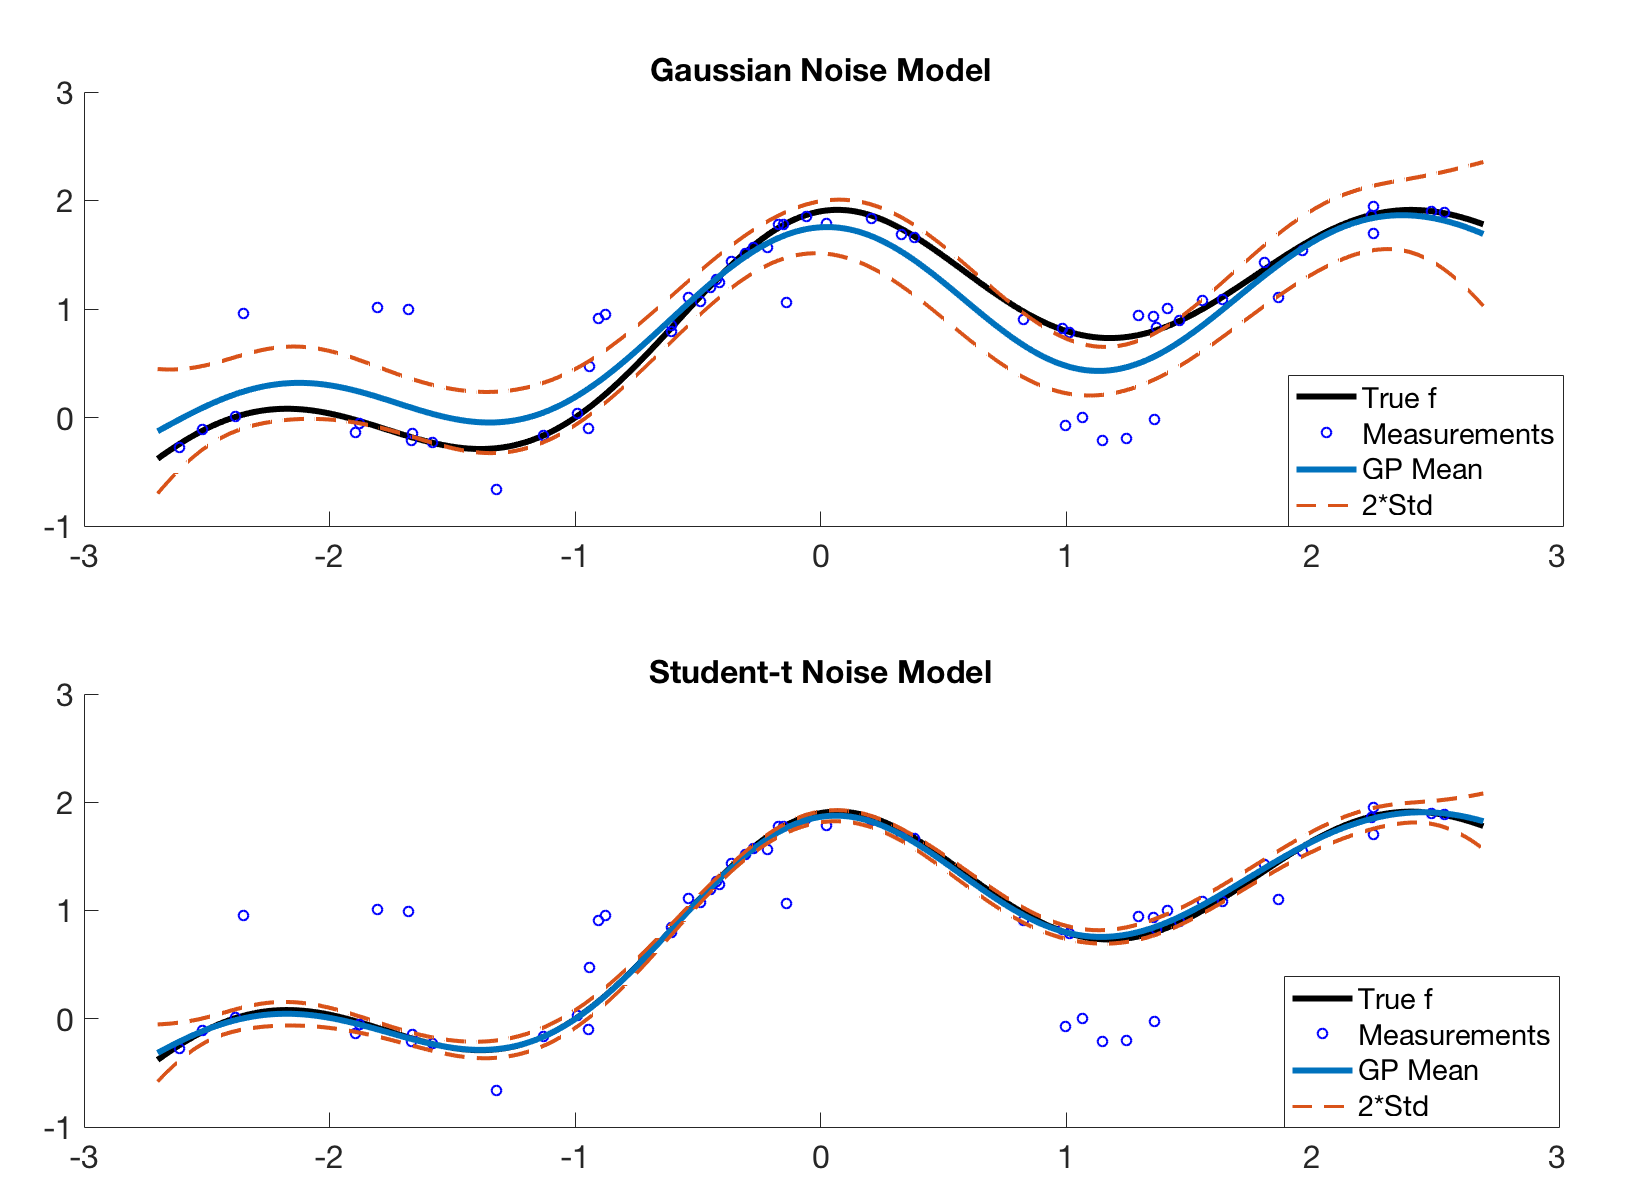
\includegraphics[width=\textwidth]{mcmcvsmap}
\caption{Gaussian MAP estimate vs. Student-t Gibbs Sampler. Data points added with Gaussian noise including some outliers with very high variance.}
\label{fig:mcmcvsmap}
\end{figure}

\section{Implementation}
There are a number of implementation choices relevant to HIL optimization. While the MCMC approach has shown to be more robust, GP regression scales linearly with the number of samples. As such, an accurate optimization of the acquisition function can take on the order of minutes. However, once a stopping condition is met the next parameter setting must immediately be communicated to the wearable device. In our implementation, we start an MCMC sampler concurrently with a new parameter evaluation. When the stopping condition is met, if the sampler has completed optimizing EI we use the returned parameter setting. Otherwise, we default to the MAP estimate to find the next parameter selection. There is then a tradeoff between the standard MAP estimate with a more robust MCMC sampler that uses one less training sample.

As Chapter \ref{ch:2} will discuss, the returned metabolic estimates have an associated variance; earlier stopping points exhibit a higher variance representing greater uncertainty for the estimated cost. The GP estimates may incorrectly inflate the best observed value if a number of parameter settings nearby are stopped early (see MAP estimate in Figure \ref{fig:mcmcvsmap} for $x\in(-2, -1)$). To appropriately weight the training samples based on their estimator variances, we fix separate noise hyperparameters corresponding to each sample. In the Gaussian noise model, the regression equation then becomes
\begin{align}
\begin{split}
  \bar{\mu}(x) &= K(X, x)^T[K(X, X) + \Sigma]^{-1}Y \\
  \bar{\sigma}^2(x) &= \kappa(x, x\vert \theta) - K(X, x)^T[K(X,X) + \Sigma]^{-1}K(X,x),
\end{split}
\end{align}
where $\Sigma$ is a diagonal matrix of entries $\{\sigma_i^2\}$ corresponding to scaled variance estimates of each data point \citep{Kersting:2007:MLH:1273496.1273546}. In the case of the MCMC model, each $y_i$ is defined independently with a noise parameter already. Figure \ref{fig:fixednoise} gives an example of the effect of fixed noise hyperparameters on the GP. Additionally, we define $y^*$ in Expected Improvement as the best mean estimate rather than the observed value. The best observed value is equally likely to be an outlier among a set of nearby points that were all measured for the full duration, so we base our decision on the variance-scaled Gaussian process estimates.

\begin{figure}[ht]
\includegraphics[width=\textwidth]{fixednoise.png}
\caption{Demonstration of the effect of fixing measurement noise. Using the same data from Figure \ref{fig:mcmcvsmap}, the noise associated with each data point is fixed and inversely proportional to the true accuracy - in effect telling the GP that the minority outliers are the more accurate values. This may arise in our stopping problem where a minimum is found (measured for the full duration, resulting variance is relatively low) and many nearby points are subsequently sampled and stopped early (resulting variances are very high).}
\label{fig:fixednoise}
\end{figure}

\chapter{Metabolic Cost Estimation}\label{ch:2}
\section{Instantaneous Energetic Cost}
The instantaneous energetic cost, our objective function, is estimated through continuous breath measurements over a lengthy duration of time. \citet{Brockway1987} developed a formula for converting $CO_2$ and $O_2$ measurements into a metabolic cost, which is then fit into a first-order dynamical model. Given the noisiness of respiratory measurements, previous studies \citep{Felt2015,Selinger2014} allowed three minutes while subjects reached a steady state before measuring for an additional three minutes to estimate an instantaneous energetic cost. In a previous Bayesian optimization study \citep{Ding2018}, each iteration used a fixed two minutes of respiratory measurements. 

Rather than requiring a fixed time interval for each evaluation, we aim to ascertain an accurate estimate only for promising parameter settings while stopping early for those that are unlikely to improve upon the best settings found so far. To make that determination, an online estimator for instantaneous energetic cost was developed using the metabolic cost model
\begin{align}
m_t(c_0, c, \tau_0, \tau) = c(1-e^{\frac{-t}{\tau}}) + c_0e^{\frac{-t}{\tau_0}},
\end{align}
where $t$ is the total measurement time in seconds and $\tau_0, \tau$ are time constants characterizing the rate of change for the initial cost $c_0$ and the instantaneous energetic cost $c$ respectively.

\begin{figure}[t]
\centering
\includegraphics[width=\textwidth]{metabolicestimation.png}
\caption{Sample estimation process for instantaneous energetic cost.}
\label{fig:metabolicestimation}
\end{figure}

\section{Parameter Estimation}
The time and cost parameters are estimated through an Unscented Kalman Filter \citep{julier1997}. Kalman filters are applied to discrete time systems of the form
\begin{align}\begin{split}
  x(t+1) &= F(x(t), v(t), t)\\
  z(t) &= H(x(t), w(t), t),
\end{split}\end{align}
where $x(t)$ represents the unobserved state of the system, $z(t)$ the observed measurement, and zero-mean Gaussian vectors $v(t)$ for process disturbances or modeling errors and $w(t)$ for measurement noise. 

First, a prediction is made for the state of the system after one timestep. Let $\hat{x}(t\vert t-1)$ represent the estimate for $x(t)$ using measurements $\mathbb{Z}(t-1)=[z(1), z(2), ..., z(t-1)]$ and $P_{x}(t\vert t-1)$ the covariance for the estimate. The prediction step aims to calculate
\begin{align}\begin{split}
  \hat{x}(t\vert t-1) &= \mathbb{E}[F(x(t-1), v(t-1), t-1)\vert \mathbb{Z}(t-1)]\\
  P_{x}(t\vert t-1) &= \mathbb{E}[\{ \hat{x}(t\vert t-1) - x(t) \} \{ \hat{x}(t\vert t-1) - x(t) \}^T \vert \mathbb{Z}(t-1)].
\end{split}\end{align}

The prediction is then reconciled with the observed measurement through a minimum mean-squared estimate $\hat{x}(t)$ and covariance $P_{x}(t)$ according to the following equations
\begin{align}
\begin{split}
  \hat{x}(t) &= \hat{x}(t\vert t-1) + Ky \\
  P_{x}(t) &= P_{x}(t\vert t-1) - KP_{y}(t\vert t-1) K^T\\
  K &= P_{xy}(t\vert t-1) P_{y}^{-1}(t\vert t-1)\\
  y &= z(t) - H(\hat{x}(t\vert t-1) , w(t), t).
\end{split}
\end{align}

The underlying requirement for these equations is an accurate propagation of the first two moments of $x(t)$ and $z(t)$. As such, Gaussian estimates are used as they assume the least information. When $F$ or $H$ is nonlinear, rather than linearizing the functions with a first order approximation the UKF approximates its probability distribution through an unscented transformation. The complete implementation details are outlined in Appendix \ref{ch:append-ukf}.

As we consider $\tau_0, \tau, c, c_0$ to be constant parameters, our UKF setup is
\begin{align}
\begin{split}
  x &= [c_0 \text{ } c \text{ } \tau_0 \text{ } \tau]\\
  F(x(t), v(t), t) &= x(t) + v(t)\\
  H(x(t), w(t), t) &= m_t(x(t)) + w(t).
\end{split}
\end{align}

\section{UKF Covariance Parameters}\label{sec:ukfcovar}
The UKF algorithm has covariance parameters $P_{x}$ for the state estimate, $P_{w}$ for measurement noise, and $P_{v}$ for process noise that determine the sensitivity of the state estimate to new measurements. Table \ref{tab:esttuningparams} summarizes the effect of increasing one of these covariance parameters while holding all others constant.

\begin{table}[h]
  \centering
  \begin{tabular}{ | c | M{10cm} |}
  \hline
  &\\
  Increase & Effect On State Estimate \\ 
  &\\
  \hline
  &\\
  $P_x$ & A higher initial covariance on the state estimate implies higher uncertainty with the state prior. Early observations will have a greater effect on the state update. However, $P_x$ decreases after every state update; observations therefore will have a smaller effect on the state estimate over time\\ 
  &\\
  \hline
  &\\
  $P_w$ & A higher measurement noise will reduce an observation's effect on the state update. The state will be slow to move away from the prior, particularly in early observations. $P_w$ also affects $P_x$ on future timesteps, as it is bounded by $P_w$\\ 
  &\\
  \hline
  &\\
  $P_v$ & While $F$ is essentially the identity function in the metabolics model as the cost and time parameters are assumed to be constant, $P_v$ encapsulates the error in that model as well as outside disturbances that can't be measured such as fatigue. Increasing $P_v$ can be used to enforce a lower bound on the effect of an observation to the state update\\ 
  &\\
  \hline

  \end{tabular}
  \caption{Tuning Parameters for metabolic estimator}
  \label{tab:esttuningparams}
\end{table}

The volatility of the estimator is dependent on the calibration of the covariance parameters with respect to the noise of the measurements. Figure \ref{fig:measurementnoise} shows three estimators: one that underestimates the measurement noise by a factor of 10, one that is exact, and one that overestimates by a factor of 10. Underestimating leads to a higher weight given to the measurement on subsequent state updates, with the volatility initially quite high. As more measurements are taken and $P_x$ decreases, the estimator eventually reaches a steady state. On the other hand, assuming too high a measurement noise will cause the estimator to slowly update towards the true value.

\begin{figure}[t]
\centering
\includegraphics[width=\textwidth]{measurementnoise.png}
\caption{With a true instantaneous energetic cost at 350 and and prior at 300, keeping all other parameters constant, the effect of using various $P_w$ values on measurement variance.}
\label{fig:measurementnoise}
\end{figure}

\section{Initial Trials and Future Work}
Using previously attained metabolic data, Figure \ref{fig:ukftuned} shows the raw and noisy measurements taken and the metabolic cost prediction that the model developed in response to a representative participant\footnote{Testing carried out by Myunghee Kim}. The bottom plot displays the covariance associated with the cost, beginning with a covariance of 1 and converging at different rates depending upon the raw data. When tuned properly, both trials see a relatively smooth rate of convergence of the estimate. With varying amounts of data provided, the accuracy in percent error was calculated by comparing with a "ground truth" value at each termination condition (5 min, 2 min, 1.5 min, 20 breaths, and 30 breaths). This ground truth value is the average of the last two minutes of data, when the subject has reached steady-state.

\begin{figure}[!ht]
\centering
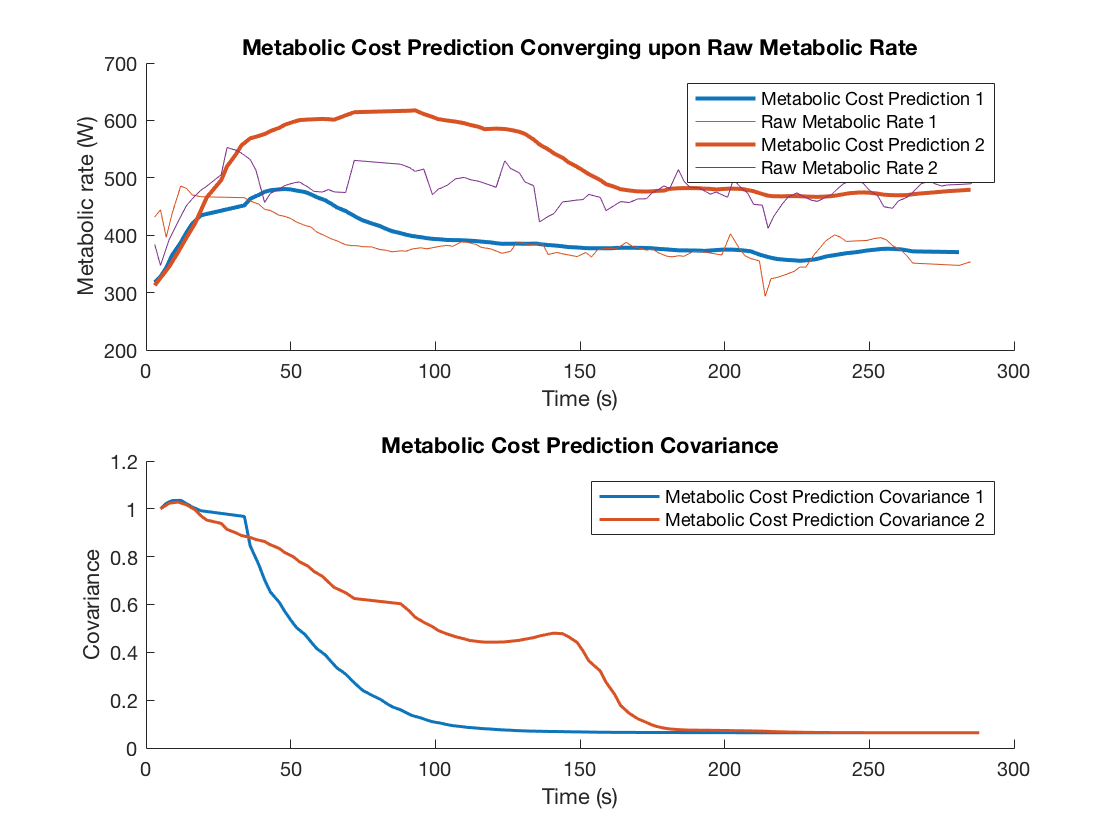
\includegraphics[width=\textwidth]{ukf}

\begin{tabular}{ |c|c|c| } 
 \hline
 Data Used & Average $R^2$ & Max \% Error \\ 
 \hline
 Full Trial & 0.996 & 0.977\% \\ 
 2 Minutes & 0.984 & 0.984\% \\ 
 1.5 Minutes & 0.973 & 0.973\% \\ 
 30 Breaths & 0.966 & 3.113\% \\ 
 20 Breaths & 0.890 & 5.767\% \\ 
 \hline
\end{tabular}%
%}
\caption{Tuned UKF Estimator over previously collected data. Accuracy assessed over partial data.}
\label{fig:ukftuned}
\end{figure}

During trial testing for our optimization methods, the same noise covariances used on the UKF estimator showed various levels of volatility across subjects (Figure \ref{fig:subjcostest}). This suggests the estimator should also have some subject-to-subject individualization based on the volatility of respiratory measurements. Future work would involve creating a cost function to optimize for this variation, balancing between the smoothness of the estimation curve and eventual convergence to the "true" instantaneous energetic cost. As Bayesian optimization starts with an exploration phase, the estimator can then be tuned a posteriori. Depending on the speed of the optimization, the estimator could potentially be tuned after every evaluation that takes the full duration, making it adaptable over time to external factors such as fatigue. Improvements in tuning the estimator would have residual effects in the information provided to both the Gaussian process and the stopping problem. Without it, Chapter \ref{ch:3} will introduce the stopping problem and different models that take into account the accuracy of the estimator. 

\begin{figure}[t]
\centering

\includegraphics[width=\textwidth]{subjcostest.png}
\caption{Tuned UKF Estimator shows different levels of volatility during optimization studies on different subjects.}
\label{fig:subjcostest}
\end{figure}

\chapter{Measurement Stopping Algorithms}\label{ch:3}
\section{Stopping Problem}
With an estimate and associated variance for the instantaneous energetic cost, the determination for when to stop measuring is known as a finite-horizon stopping problem. Formally, the stopping problem is defined with

\begin{table}[h]
\centering
\begin{tabular}{ |c  c| }
  \hline&\\
  $N$ & Finite horizon\\
  &\\
  $X_t$ & State at time $t$\\
  &\\
  $P(X_t \vert X_{t-1})$ & State transitions, typically Markovian\\
  &\\
  $\lambda$ & Discount Factor $\in (0, 1]$\\
  &\\
  $r(X)$ & Bounded reward function for continuing at state $X$\\
  &\\
  $g(X)$ & Bounded reward function for stopping at state $X$\\
  &\\
  \hline
\end{tabular}
\caption{Setup of finite horizon stopping problem}
\label{tab:stopping}
\end{table}

The objective is to find $\tau$ that maximizes
\begin{align}
  V(x) = \max_{\tau: \tau \leq N} \mathbb{E}[\lambda^{\tau} g(X_{\tau}) + \sum_{i=0}^{\tau-1} \lambda^{i}r(X_j) \vert X_0 = x].
\end{align}

The value function can be computed via backward induction by defining
\begin{align}
\begin{split}
  J_N(x) &= g(x)\\
  J_n(x) &= max\{g(x), r(x) + \lambda\mathbb{E}_{P(y\vert x)}[J_{n+1}(y)]\},
\end{split}
\end{align}
then $V(x) = J_0(x)$ and the optimal stopping time is
\begin{align}
  \tau = \min_{t \geq 0}J_t(X_t) = g(X_t).
\end{align}
For a derivation of the optimal stopping time, see Appendix \ref{thm:ost}. We aim to formulate the stopping problem in terms of the metabolic estimator. Let $N$ be the maximum measurements allowed at a parameter evaluation, $\hat{x}_t \sim \mathcal{N}(\mu_{x_t}, \sigma^2_{x_t})$ the cost estimate and associated variance for the current evaluation, and $\hat{x}^* \sim \mathcal{N}(\mu_{x^*}, \sigma^2_{x^*})$ the cost estimate and variance for the best parameter setting found thus far as defined by the Gaussian process. As Bayesian optimization starts with an exploration phase, $\hat{x}^*$ will always be defined (Algorithm \ref{alg:bayesopt}).

\section{$\sigma$-scaled Offset}
The $\sigma$-scaled offset model directly embeds $\hat{x}_t$ and $\hat{x}^*$ into the stopping problem. The best estimate of the difference in energetic costs is given by the following Gaussian distribution
\begin{align}
\begin{split}
  \hat{x}_t - \hat{x}^* &\sim \mathcal{N}(\mu, \sigma^2)\\
  \mu &= \mu_{x_t} - \mu_{x^*}\\
  \sigma^2 &= \sigma^2_{x_t} + \sigma^2_{x^*}.
\end{split}
\end{align}

The stopping problem state is then the estimate difference, with a non-Markovian transition model of independent draws from the same Gaussian distribution. The lower $x_t$ seems relative to $x^*$, the higher the reward function incentivizes continuing. In summary,

\begin{align}
\begin{split}
  X_t &= \mu\\
  P(X_t \vert X_{t-1}) &= P(X_t) \sim \mathcal{N}(\mu, \sigma^2)\\
  r(x) &= K\sigma-x\\
  g(x) &= 0,
\end{split}
\end{align}
where $K$ is a $\sigma$-scaled offset to provide some risk averseness to the estimate. The optimal stopping point for this formulation can be characterized as the first time $X_t > K\sigma$. As more measurements are taken and $P_{x}$ decreases, $\sigma^2$ decreases the offset accordingly.

As shown in Section \ref{sec:ukfcovar}, underestimating $P_w$ can cause the estimator to exhibit high volatility. Additionally, since a subsequent state covariance update $P_x(t+1)$ is bounded by $P_w$, a lower $P_w$ will also cause $\sigma^2$ to be underestimated. With the $\sigma$-scaled offset model, underestimating the noisiness of observations could potentially cause promising parameter settings to stop measuring early as there is no fault tolerance for crossing the threshold. 

\section{Gittins Index}
A more fault-tolerant model is drawn from literature related to the multi-armed bandit problem (MAB), which represents a sequential decision making problem where at any given time a player must select from different options (or arms) that then responds with a variable reward. Historically this has been used in a clinical context, where a physician must select from one of several different treatment options when presented a patient and receives binary rewards of either successes or failures \citep{Villar2015}. A stopping problem has also been described as a one-armed bandit problem \citep{FergusonStopping2006}.

Successes and failures can be based on $\mu, \sigma^2$ using the Probability of Improvement (PI) metric
\begin{align}
  PI(\mu, \sigma^2) = \Phi(\frac{\mu}{\sigma}),
\end{align}

where $\Phi$ is the CDF for a standard normal distribution. A success can then be defined as $PI(\mu, \sigma^2) > T$ for some defined risk tolerance measure $T$. As $\sigma^2$ decreases over more measurements, $PI$ becomes less influenced by $\sigma^2$ and more by $\mu$. 

The stopping problem state follows a Beta distribution where parameters $\alpha,\beta$ correspond to the count of successes and failures, and transitions follow the posterior of the Beta distribution. In summary,
\begin{align}
\begin{split}
  X_t &= (\alpha_t + \alpha_0, \beta_t + \beta_0) \\
  P(X_{t+1}) &=
  \begin{cases}
      (\alpha_t + \alpha_0 + 1, \beta_t + \beta_0)
      \\ \tab\text{w.p. } \frac{\alpha_t + \alpha_0}{\alpha_t + \alpha_0 + \beta_t + \beta_0}\\
      (\alpha_t + \alpha_0, \beta_t + \beta_0 + 1)
      \\ \tab\text{w.p. } \frac{\beta_t + \beta_0}{\alpha_t + \alpha_0 + \beta_t + \beta_0}
  \end{cases}\\
  r(X_t) &= \frac{\alpha_t + \alpha_0}{\alpha_t + \alpha_0 + \beta_t + \beta_0},\\
\end{split}
\end{align}
where $\alpha_0,\beta_0$ are smoothing priors and $\alpha_t,\beta_t$ are successes and failures up to time $t$.

Gittins and Jones showed that an optimal policy could be constructed by calculating a value called the Gittins Index \citep{doi:10.1002/9781118596333.ch24}. Let $g(x) = K$ for some constant $K$, then the Gittins Index is defined as
\begin{align}
  \nu(X_t) = (1-\lambda)\min_{K} \{J_t(X_t) = K\}.
\end{align}
The Gittins Index is generally used for infinite horizon stopping problems, with $g(x)=\frac{\nu(x)}{1-\lambda}$ representing an infinite geometric sum to compensate for all future rewards. By setting $\lambda=1-\frac{1}{N}$, $\forall x \; 0 \leq \nu(x) \leq 1$.

In the case of a multi-armed bandit problem, the optimal policy is to play the arm with the highest Gittins Index. \citet{FergusonStopping2006} shows that the stopping problem, or the one-armed bandit problem, is equivalent to having a second arm that provides a constant reward. The optimal policy then corresponds to playing the arm as long as its Gittins Index is above a specified threshold $V$. As $T$ and $V$ are correlated, one of the parameters can be fixed (such as $T=0.5$) while the other is tuned to a preferred risk tolerance for expected success rate. 

This approach essentially acts as a low-pass filter for a potentially noisy metabolic estimator. The choice for $V$ can similarly be thought of in terms of a Gittins Index 
\begin{align}
\begin{split}
  \nu((\alpha, \beta)) &= V\\
  \alpha + \beta &= N,
\end{split}
\end{align}
where $\alpha, \beta$ are successes and failures over the maximum duration. This is in essence asking the question: "If I were to continue measuring this parameter setting, what is the minimum number of successes that I would need to warrant the cost of experimental time?".

\section{Adaptive Thresholds}
Both the $\sigma$-offset and Gittins model have a risk tolerance threshold that may be difficult to tune across subjects. Another approach is to use the exploration phase of Bayesian optimization to create a schedule for the thresholds adapted to the subject's measurements. A simple approach would be to gauge the trajectory of thresholds if the stopping problem were run on the exploration phase, and accordingly use the most risk averse during the optimization. Let $M$ and $\Sigma$ be $\vert \mathbb{E}\vert \times N$ matrices providing traces where $M_{ij}, \Sigma_{ij}$ correspond to $\mu_{x_j}, \sigma^2_{x_j}$ for exploration point $i$ and measurement $j$. For each exploration point, the $\hat{x}^*$ distribution can be the final distribution, $(M_{iN}, \Sigma_{iN})$, to estimate the magnitude of thresholds when comparing similar cost estimates. Algorithm $\ref{alg:adapthresh}$ details the calculation of a threshold vector $A$.

\begin{algorithm}[t]
\caption{Determining threshold levels for either model based on subject's exploration data. With the $\sigma$-offset, the higher threshold is more risk averse, while with the Gittins model the lower is.}
\label{alg:adapthresh}
\begin{algorithmic}
\State \textkeyword{Init $\vert\mathbb{E}\vert \times N$ Matrix } $X$
\State \textkeyword{Init $N$-Vector } $A$
\State \textkeyword{Define Window } $W$
\For{i=1}{\vert \mathbb{E} \vert}
  \State $\alpha = \alpha_0, \beta = \beta_0$
  \For{j=1}{N}
    \State $\mu = M_{ij} - M_{iN}$
    \State $\sigma^2 = \Sigma_{ij} + \Sigma_{iN}$
    \If{Offset}
      \State $X_{ij} = \frac{\mu}{\sigma}$
    \EndIf
    \If{Gittins}
      \State $\alpha = \alpha + \mathbb{1}_{PI(\mu, \sigma^2) \geq T}$
      \State $\beta = \beta + \mathbb{1}_{PI(\mu, \sigma^2) < T}$
      \State $X_{ij} = \nu((\alpha, \beta))$
    \EndIf
  \End
\End
\For{i=1}{N}
  \If{Offset}
    \State $A_{i} = MAX\{X_{rc}\vert 1 \leq r \leq \vert\mathbb{E}\vert, i-W \leq c \leq i+W\}$
  \EndIf
  \If{Gittins}
    \State $A_{i} = MIN\{X_{rc}\vert 1 \leq r \leq \vert\mathbb{E}\vert, i-W \leq c \leq i+W\}$
  \EndIf
\End
\State Return $A$
\end{algorithmic}
\end{algorithm}

\section{Simulations}
Simulations were run on four optimization functions (Table \ref{tab:optfunc}) with Gaussian noise added proportional to the standard deviation of the respective function. The Hartmann-6 and Ackley functions have larger domain spaces with lower standard deviations, generally making them more difficult functions to optimize using Bayesian optimization. While the Levy and Branin functions have large regions of local minima, and in Branin's case three global minima, much higher noise is added due to the standard deviations of the respective functions.

\begin{table}[t]
\centering
\begin{tabular}{ |c | c | c | c | c | }
  \hline&&&&\\
  Function & Domain & Minimum & Mean & Std\\
  &&&&\\
  \hline
  &&&&\\
  Hartmann-6 & $[0,1]^6$ & -3.322 & -0.259 & 0.383\\
  &&&&\\
  Ackley & $[-32.768, 32.768]^4$ & 0 & 20.882 & 1.027\\
  &&&&\\
  Levy & $[-10, 10]^4$ & 0 & 42.544 & 27.939\\
  &&&&\\
  Branin & $([-5, 10],[0, 15])$ & 0.398 & 54.452 & 51.129\\
  &&&&\\
  \hline
\end{tabular}
\caption{Optimization functions for simulations}
\label{tab:optfunc}
\end{table}

Both the $\sigma$-offset and Gittins models were tested each with risk thresholds $T=[0, 0.25, 0.5, AD]$ where $AD$ is the adaptive threshold method. A Gaussian state estimate was continually reconciled with new observations, equivalent to a Kalman filter with the identity function plus additive noise for both $F$ and $H$, and measurement noise was tuned to different scenarios $P_w=[\frac{\sigma^2}{10}, \sigma^2, 10\sigma^2]$. $P_x$ was initialized to $\mu, \sigma^2$ of the function, and $P_v=\frac{\sigma^2}{100}$. The same observations from exploration points were provided for each function under all scenarios, and the maximum duration was set to 45 measurements.

For time $t$, let $x_t$ be the GP's estimated minimum point. The figures chart
\begin{align}
  y_t = \frac{f(x_t) - f(x^*)}{f(x_0) - f(x^*)},
\end{align}
where $f$ is the true, noiseless function and $f(x^*)$ is the function minimum.

Results from simulations averaged over 100 trials are provided in Appendix \ref{ch:append-sims}. The exploration phase is omitted from the figures as the same observations were used for all scenarios, though final estimates may vary across different $P_w$ values. The case of $T=0$ for the Gittins model is equivalent to a fixed measurement window and can be used as the point of comparison. Stopping early shows a clear benefit in Hartmann and Ackley, the less noisy functions. The $\sigma$-offset method generally outperforms the Gittins in these situations, and is comparable only to the most aggressive $T=0.5$ case. As there is minimal noise, different levels of $P_w$ show only slight differences. 

In the case of higher noise with Branin and Levy, only Levy shows a clear advantage to stopping early. With the more fault-tolerant Gittins approach, different levels of $P_w$ still show relatively consistent performance, while having a constant threshold in the $\sigma$-offset model quickly stagnates when underestimating measurement noise. Note these functions are not strictly decreasing - this implies a training sample has been added that causes the Gaussian process to incorrectly assume a new minimum point. As $P_w$ increases this becomes less apparent; a higher $P_w$ causes $\sigma^2$ of the model to also increase, and as both models are $\sigma$-scaled the thresholds are rarely met until a more refined estimate is made. 

The adaptive thresholds show fairly consistent performance across all scenarios, including with underestimating $P_w$ in the $\sigma$-offset model. Generally a higher $P_w$ estimate allows for a more predictable trajectory, which makes the adaptive thresholds more effective. In these experiments, eight exploration points were used, making the exploration phase one third of the entire trial time. Additional tests would include decreasing the number of exploration points, especially in the case of underestimating $P_w$ with either the Branin or Levy functions, and altering the maximum duration window.

To date, wearable devices have shown to provide a metabolic reduction on the order of twenty percent. The standard deviation in metabolic rate across parameter settings, while heavily subject dependent, has ranged from ten to thirty percent across our trials so far, making the Branin and Levy functions a more appropriate comparison. Though difficult to measure the noisiness of metabolics as there is no true instantaneous energetic costs to compare against, the importance of the relative magnitudes between $P_w$ and $P_x$, $P_v$ are clear in both affecting the stopping process as well as Gaussian process estimates. The bandit model aims to reduce the effect of incorrectly assigning values to these covariances, while the $\sigma$-offset model generally performed the best when tuned properly.

\chapter{Subject Trials}\label{ch:4}
\section{Experimental Protocol}
\subsection*{Optimization Parameters}
An initial pilot was run varying 6 parameters
\begin{table}[h]
  \centering
  \begin{tabular}{ c c }
  Peak Force & Maximum force in Newtons provided\\
  Onset Timing & Start of assistance during the gait cycle\\
  Peak Timing & Point of peak force provided during the gait cycle\\
  Offset Timing & End of assistance during the gait cycle\\
  Curvature 1 & Force provided at midpoint of onset and peak\\
  Curvature 2 & Force provided at midpoint of peak and offset
  \end{tabular}
\end{table}

\subsection*{Hip-only Soft Exosuit}
The textile components of the hip-only soft exosuit consist of a short spandex base layer, a waist belt, and two thigh braces as described in \citep{Lee2018}. Two IMUs (MTi-3 AHRS, Xsens Technologies B.V., Enschede, Netherlands) mounted on the anterior part of the thigh measure the orientation and angular velocity of thigh segments which are used for gait cycle estimation in real-time \citep{Ding2016}. The anchoring points of the Bowden cable are at the bottom left and right of the waist belt as well as at the middle center of the thigh braces from the posterior view. Two load cells (LSB200, Futek Advanced Sensor Technology Inc., CA, USA) are integrated in the aluminum attachment piece of the anchoring point to measure the cable force. When the actuator pulls the inner cable, the soft exosuit generates a hip extension torque by shortening the distance between two anchoring points. 

\subsection*{Actuation System}
The two DOF actuators in the off-board system are used to deliver hip extension assistance to both legs. Each actuator consists of a customized brushless motor (Allied Motion, Colorado, USA), a 9.25:1 spiroid gear set (ITW Heartland, MN, USA) and a 45 mm radius pulley. The pulley groove is designed to be able to wrap the inner Bowden cable 1.5 times around the pulley, allowing 420 mm of cable travel \citep{Lee2018}. A 360 counts/rev incremental encoder (AS5134-ZSST, ams AG, Premstaetten, Austria) is mounted on the customized motor to measure its position and velocity. The Bowden cable sheath of the actuator side connects to the pulley cover and inner cable attaches to the pulley. When the motor rotates, the actuator can either pull in the inner cable to generate a force or push the cable out so it can go slack.

\subsection*{Control System Architecture}
The electronics hardware has a three-layer configuration for the control system architecture: real-time target machine (top layer), microprocessor (middle layer), and servomotor driver (bottom layer). In the top layer, the Speedgoat real-time target machine runs a Simulink model in a host laptop. A PCI interface card (CAN-AC PCI, Softing AG, Haar, Germany) for CAN communication is installed on the target machine to acquire sensor signals and send the command to the servomotor driver through the microprocessor. The microprocessor (Due, Arudino, Ivrea, Italy) in the middle layer acts as a signal hub between target machine and servomotor driver while protecting the system from undesired behavior of the actuator due to anomalous errors from the target machine. In the bottom layer, Gold Twitter (Elmo Motion Control Ltd, Israel) with 55V maximum supply voltage and 60 A peak current is selected as the current servomotor driver. It tracks the current command from the microprocessor to drive the actuator. The CAN communication between layers closes the control loop at 1kHz loop rate \citep{Lee2018}.

Another laptop collects the metabolic data, runs an optimization algorithm, and sends the assistance profile parameters that will be explored in the next condition to the host laptop. Ethernet communication is used between a real-time target machine, a host laptop, and the second laptop. Based on the profile parameters calculated by the algorithm, the host laptop sends the current command to the servomotor drive to deliver assistance to the subject.

\section{Experimental Subjects}
Two male subjects (S1: 27 yrs, 74 kg, 177 cm; S2: 48 yrs, 85 kg, 178 cm) participated in this preliminary study. The subjects walked on the treadmill at 1.25 m/s under four different conditions: Normal walking without Exosuit (N), Exosuit-off (OFF), Fixed Exosuit Assistance (FIX) and Optimal Exosuit Assistance (OPT). During FIX condition, the force profiles assisting hip extension were based on the previous study of \citep{Ding2016}, whereas force profiles in OPT condition were determined through a two-part procedure (8 exploration points, 5 minute break, then 40 minute continuous optimization) which was performed before walking test conditions. Metabolic cost of walking across different conditions was measured using a portable gas analysis system (K4b2, Cosmed, Roma, Italy).

\begin{figure}[t]
\centering
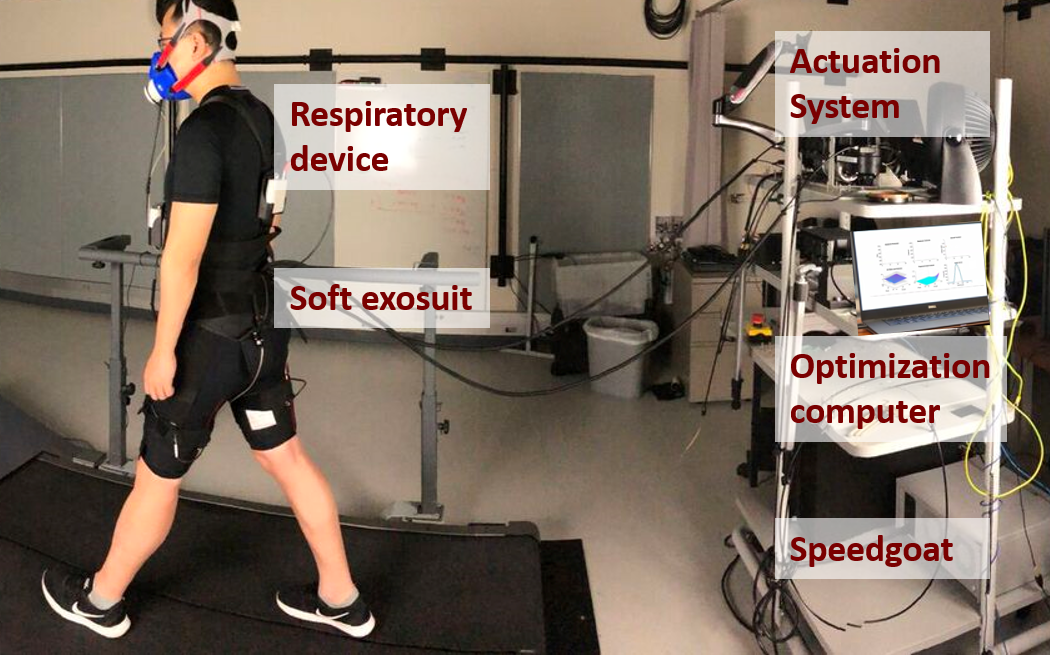
\includegraphics[width=\textwidth]{system_setup.png}
\caption{Experimental setup. Assistance parameters for the soft exosuit were optimized on-line. Respiratory device measured respiratory rate to estimate metabolic cost for a given condition with a covariance. In the optimization computer, the Gittins process determined when to stop sampling and Bayesian optimization was used to select a next parameter set. The parameters were sent to the real-time computer (speedgoat) to generate a force trajectory. Then, the actuator provided a force to a subject through a bowden cables. }
\label{fig:expsetup}
\end{figure}

\section{Results}
Two human trials with the same subjects from a previous study were conducted as a comparison. The Gittins method was used with a relatively risk averse $K=0.35$ to account for the possibility of a very low signal-to-noise ratio, as well as the practical consideration of parameters requiring time to fully propagate to the suit. A summary of the metabolic reduction can be found in Table \ref{fig:expsummary} with figures for the optimized force assistance in Figure \ref{fig:forceprofile}. The soft exosuit followed desired trajectory within 5\% error, relative to the peak force.

\begin{figure}[t]
\centering
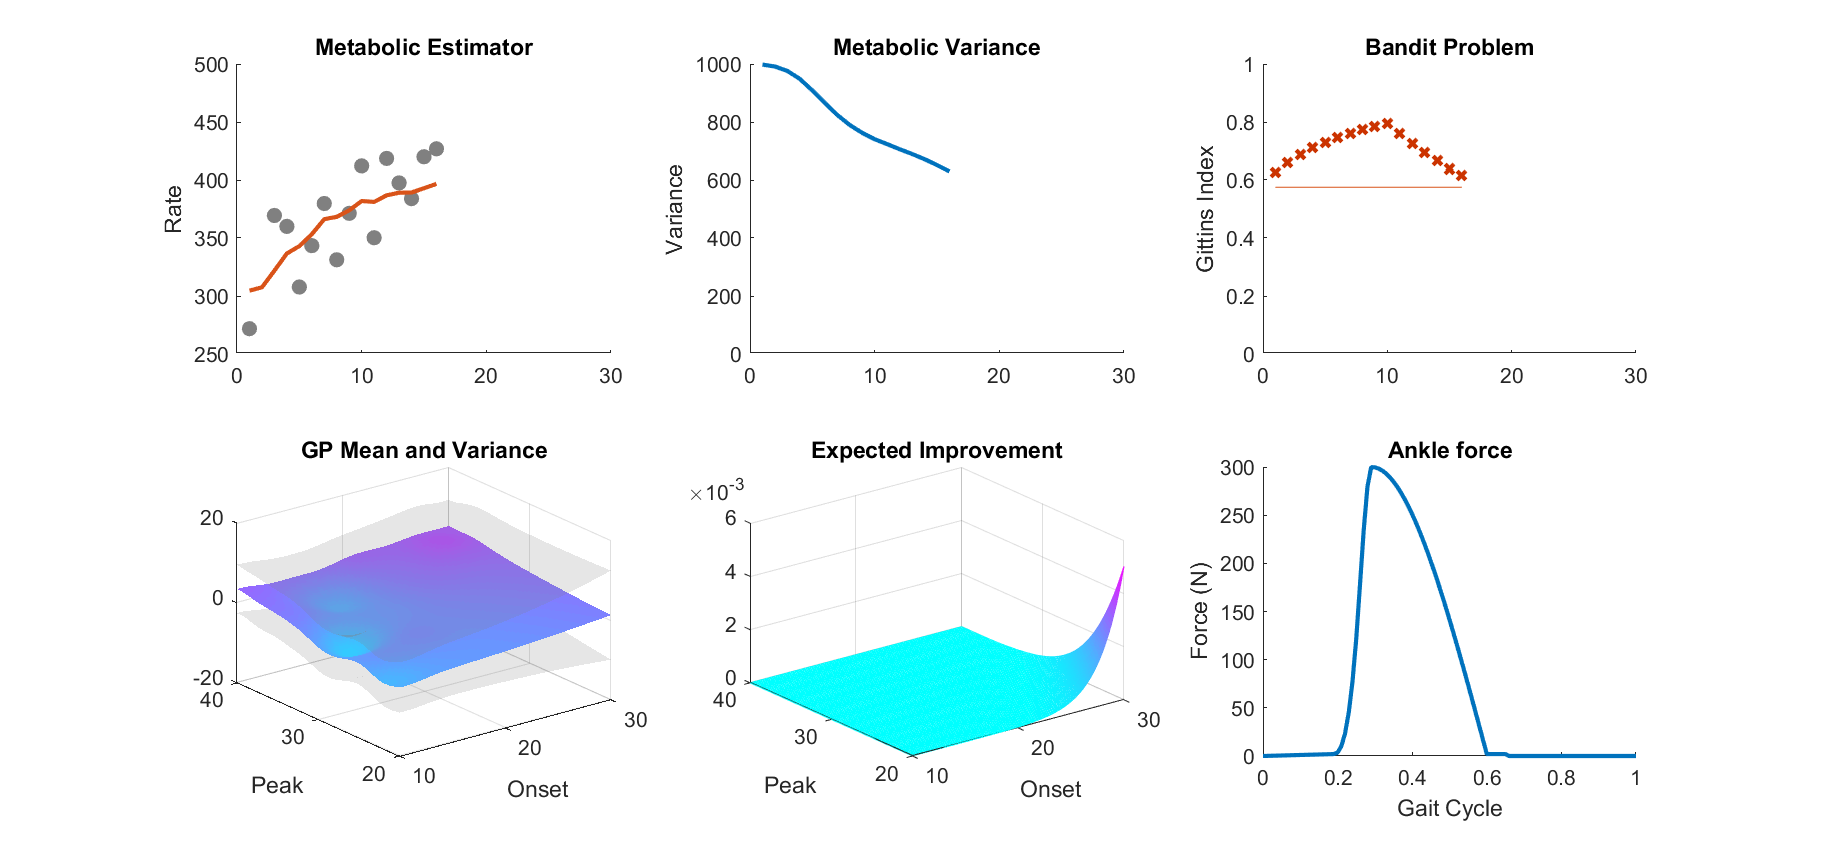
\includegraphics[width=\textwidth]{block}
\caption{Diagram of Bandit Process}
\label{fig:block}
\end{figure}

\begin{table}
\centering
\begin{tabular}{ |c|c|c|c|c|c|c| } 
 \hline
 Subj & OPT & FIX & OPT Peak F & FIX Peak F\\ 
 \hline
 1 & 35\% & 29\% & 223N & 247N\\
 2 & 7\% & -4\% & 174N & 230N \\
 \hline
\end{tabular}%
\caption{Subject Trial Summary}
\label{fig:expsummary}
\end{table}

\begin{figure}[t]
\centering
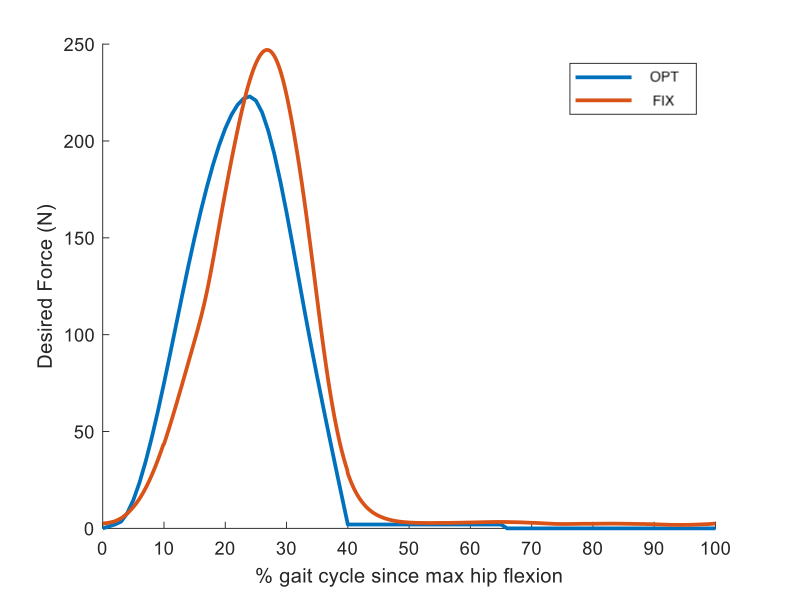
\includegraphics[width=.5\linewidth]{subj1}\hfill
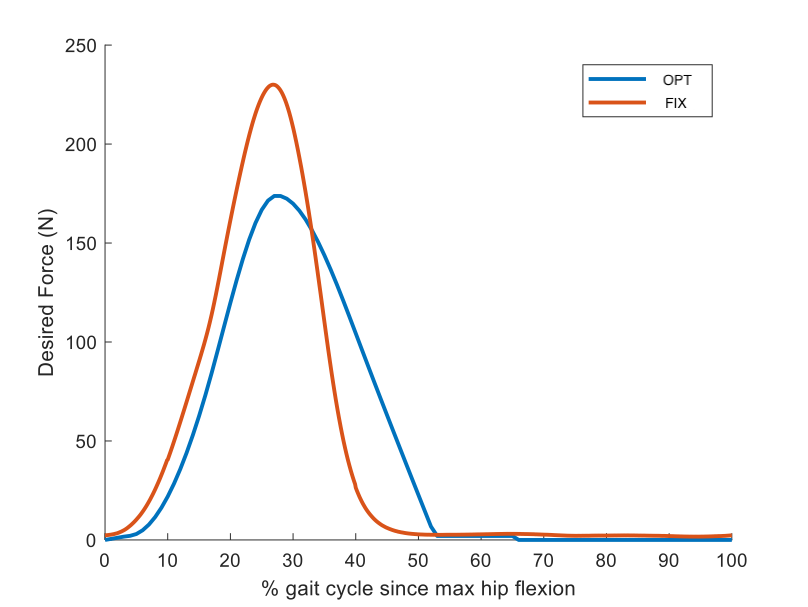
\includegraphics[width=.5\linewidth]{subj2}
\caption{Force profiles of the two subjects}
\label{fig:forceprofile}
\end{figure}

\section{Conclusions}
A new metabolic estimator based off the Unscented Kalman Filter algorithm was designed to enable early stopping for a parameter evaluation. The estimator has shown the ability to track the instantaneous metabolic rate online with varying amounts of data, but is sensitive to the parameterization of it's covariance matrices. Two methods were developed for early stopping: a simple $\sigma$-offset threshold strategy and a bandit process strategy based off the Gittins Index. Depending on the noisiness of the estimator, the bandit process provides a higher fault tolerance for noisy observations. Two trials were then conducted using the Gittins algorithm to optimize over six hip parameters and we found comparable metabolic reduction to a previous study with the same subjects. In the previous study ample time was spent isolating the parameters individually to find the two with high variability (peak and offset timing). While the optimization period for a trial is slightly longer, we were able to find similar results without the need for an extensive pre-trial exploration phase. Interestingly, we also found a lower peak force to provide similar metabolic reduction in each of the two subjects. Having a lower peak force could provide two benefits: lower battery requirements on the suit and more importantly reduced strain on the harness and subsequent discomfort to the user. Future work in this area can focus on tuning the estimator's covariance matrices with exploration phase data and testing more subjects with both models. In particular, an area of interest would be using the algorithm in multi-joint optimization \citep{1298569}.

\chapter*{Conclusion}\label{ch:concl}
\subsection*{Summary}
This thesis aims to introduce a stopping criteria for measurement time within HIL optimization. A metabolic estimator based off the Unscented Kalman Filter algorithm was designed and has effectively shown the ability to track the instantaneous energetic cost online with varying amounts of data. Two methods were developed for early stopping: a simple $\sigma$-offset threshold strategy and a bandit process strategy based off the Gittins Index. Depending on the noisiness of the estimator, the Gittins approach can provide a higher fault tolerance for noisy observations. Bayesian optimization with a Gaussian process prior was used as an overall design framework for selecting parameter settings to sample from. Two trials were then conducted using the Gittins approach to optimize over six hip parameters and similar metabolic reduction was achieved compared to a previous study with the same subjects. While the previous study had a shorter duration time, it was only a two-parameter study and ample time was spent prior to the subject tests isolating the parameters individually to find the two with highest variability (peak and offset timing). In our case, we were able to find similar results without the need for an extensive pre-trial exploration phase. Interestingly we also found a lower peak force to provide similar metabolic reduction in each of the two subjects. Having a lower peak force provides two benefits: lower battery requirements on the suit and reduced strain on the harness and subsequent discomfort to the user.

\subsection*{Challenges and Future Work}
There were a number of implementation choices that can be improved upon in future work. While collecting ample metabolic data is a time-constrained challenge, in the future a prior metabolic landscape could potentially be developed as a mean function for the Gaussian process. With respect to the Bayesian optimization, accounting for the early stopping of parameter settings led to fixed noise hyperparameters based off the metabolic estimator. Alternatively, a fully heteroscedastic approach could be experimented with that involves fitting output noise to a secondary Gaussian process. For the metabolic estimator, the high subject-to-subject variability in measurements requires some optimization for the covariance matrices. Given Bayesian optimization has an exploration phase, tuning the estimator based on this data should improve reliability. Similarly, different methods for tuning the risk tolerances of the stopping algorithms could be analyzed through additional subject tests. Two subject trials is certainly not enough, and many more subject tests should be carried out for a better analysis of the stopping algorithms in practice. Finally, an area of current interest is multi-joint optimization using both ankle and hip actuation \citep{1298569}. This would be a natural use case for the stopping algorithm as the number of optimization parameters could potentially double. Current pilot tests are being run optimizing four parameters: peak timing in both the hip and ankle, onset timing in the ankle, and offset timing in the hip.

%%%%%%%%%%%%%%%% BACK MATTER %%%%%%%%%%%%%%%%

% Put appendices, bibliography, and supplemental materials here

% The bibliography may be single spaced within each entry, but must be
% double-spaced between each entry. Most bibliography styles leave space between
% entries, so that shouldn't be a problem.
\begin{singlespacing}
  % I like "References" better than "Bibliography"
  \renewcommand{\bibname}{References}

  % Any bibliohgraphy style that leaves space between entries is fine
  \bibliographystyle{ecca}
  \bibliography{references}
\end{singlespacing}

% Appendices from all chapters should go at the end
\begin{appendices}

\chapter{Bayesian Optimization}

\begin{sidewaysfigure}[h]
\begin{subfigure}{\textwidth}
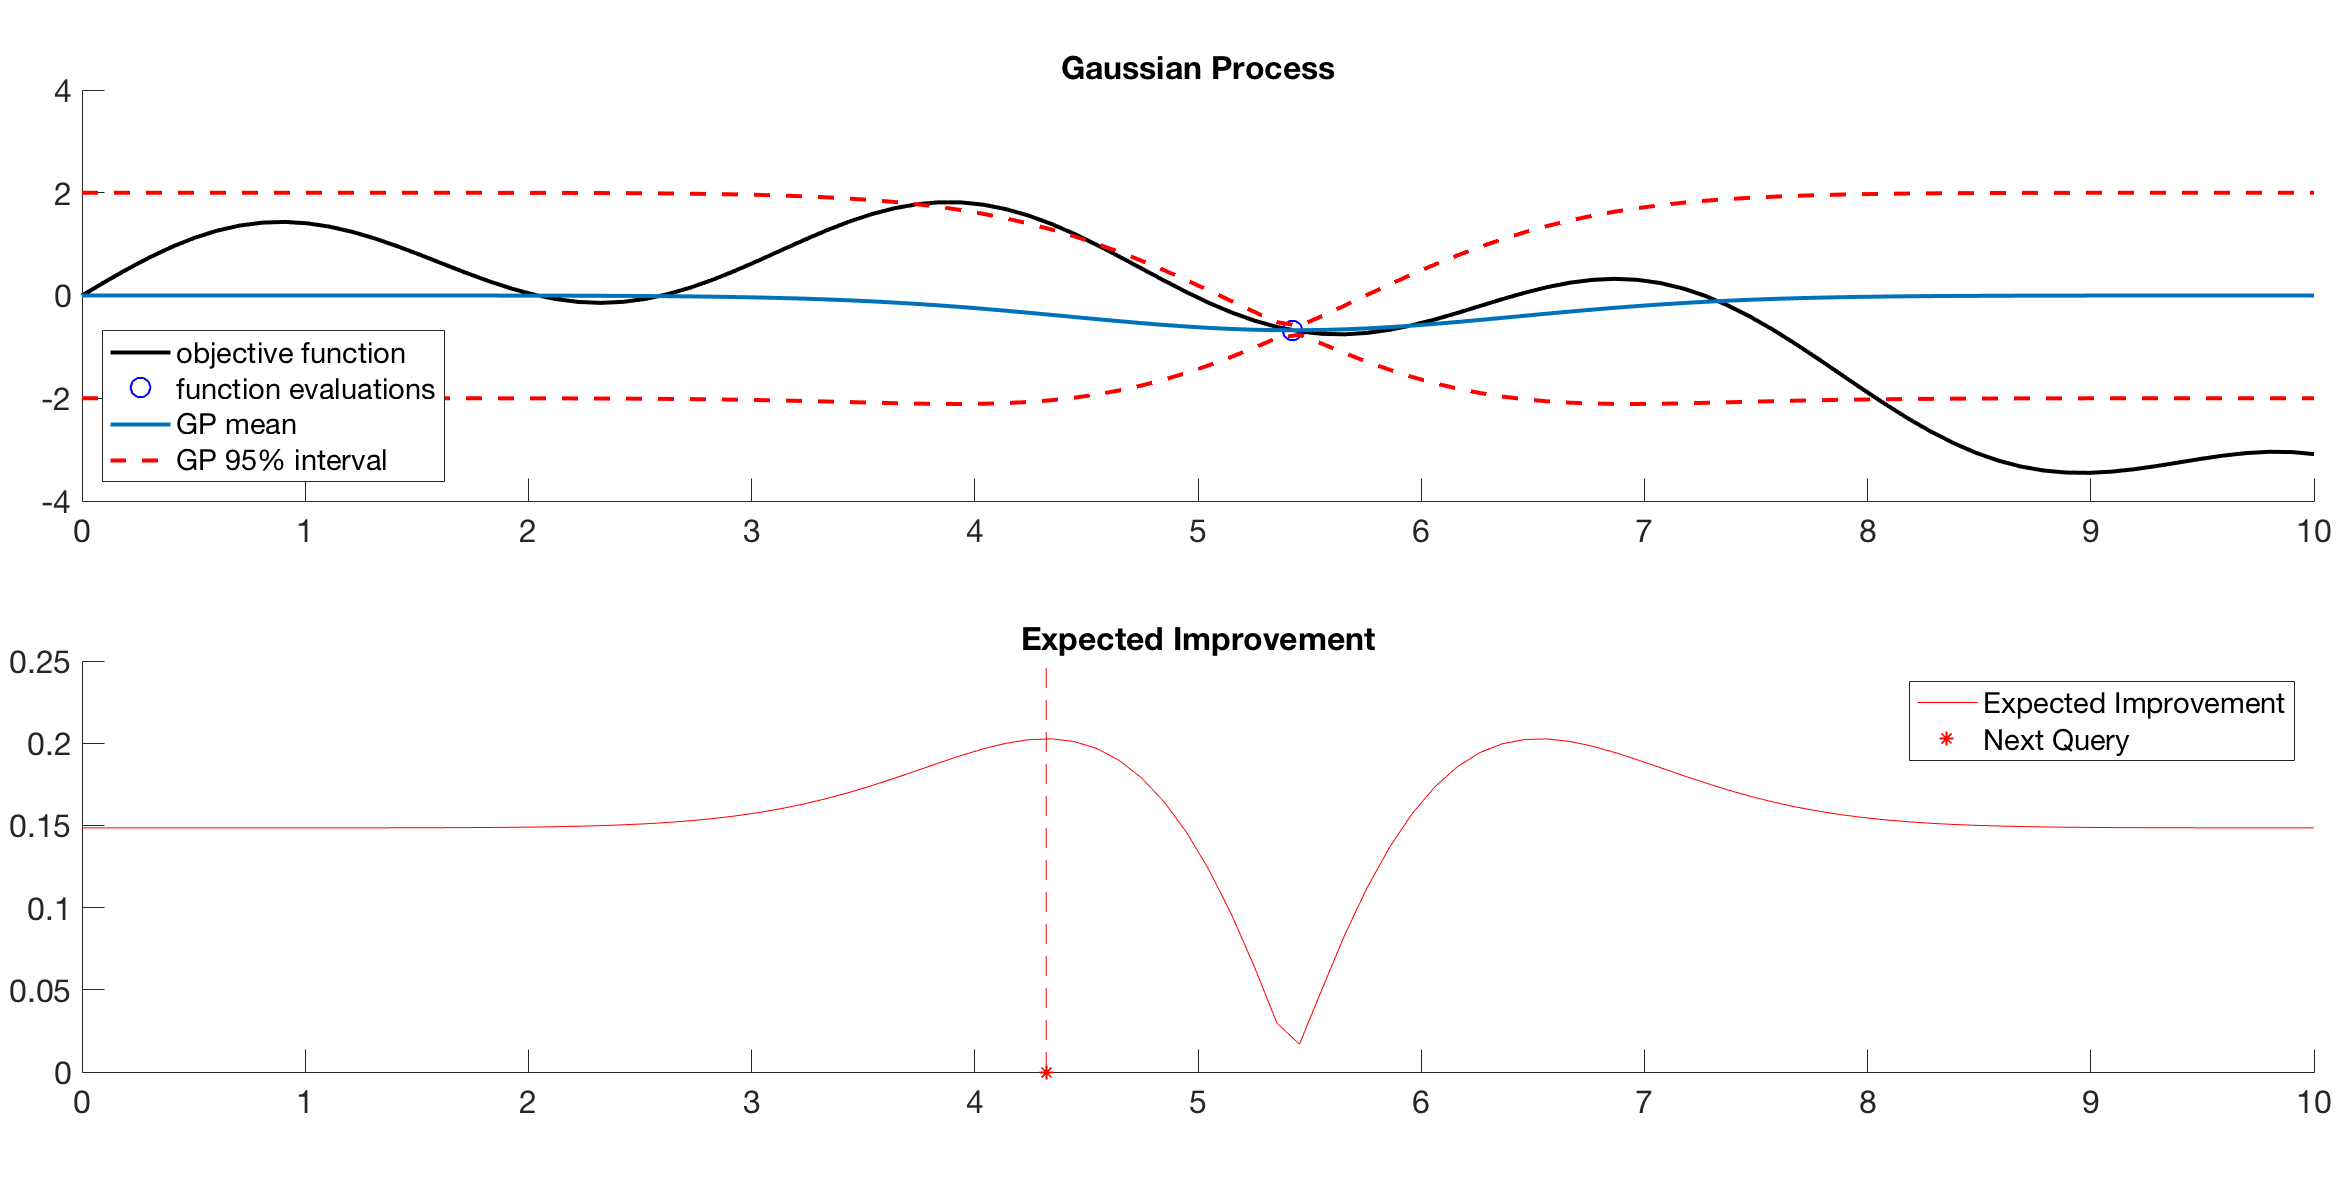
\includegraphics[width=.5\textwidth]{ei1.png}\hfill
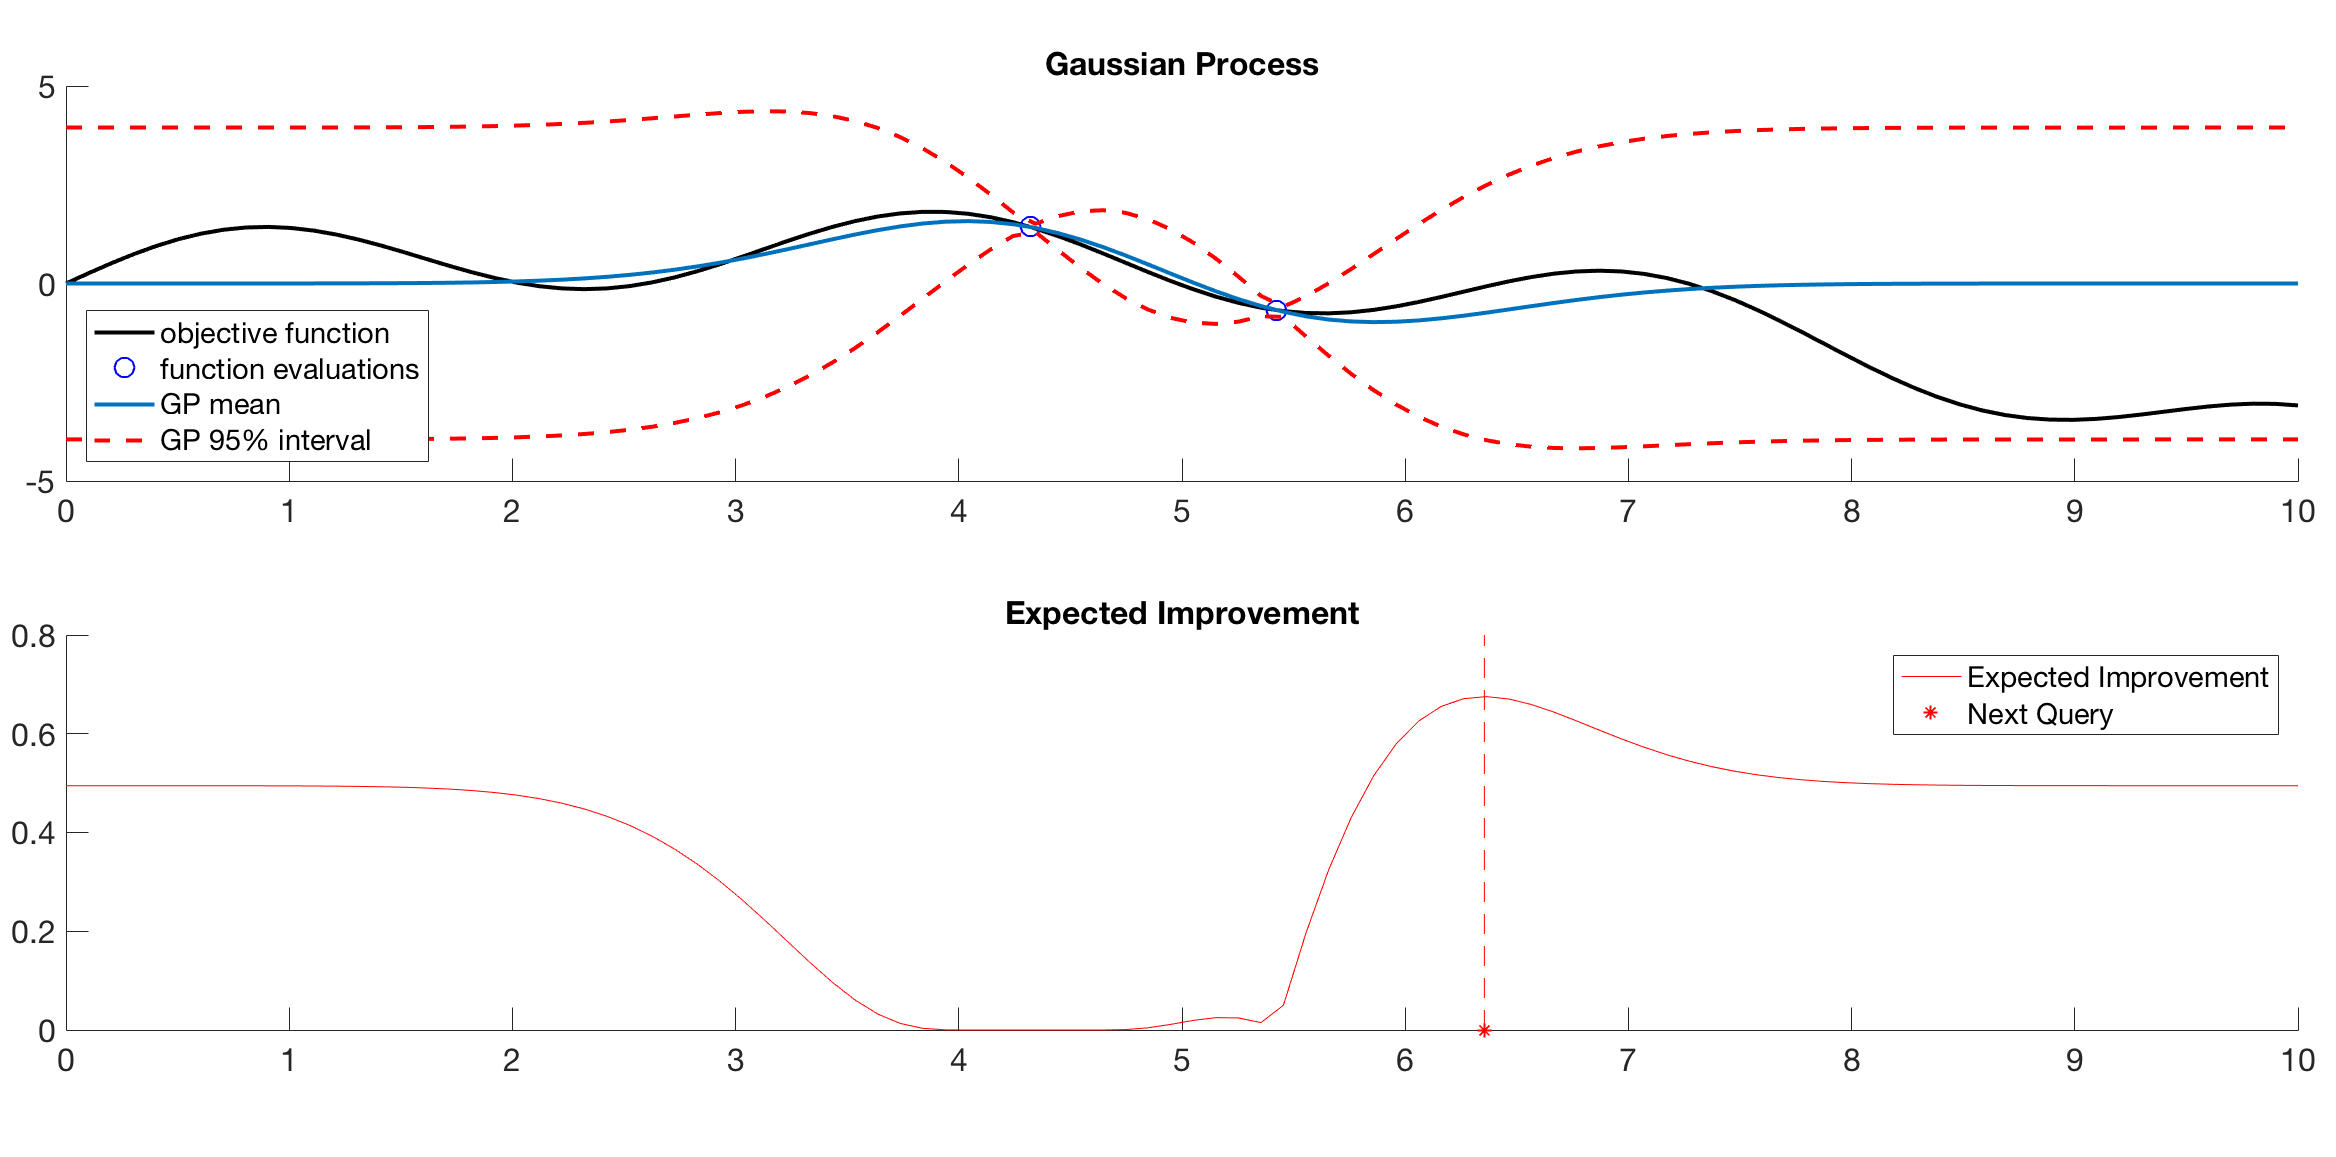
\includegraphics[width=.5\textwidth]{ei2.png}
\caption{Iterations 1 and 2}
\end{subfigure}
\par\medskip
\begin{subfigure}{\textwidth}
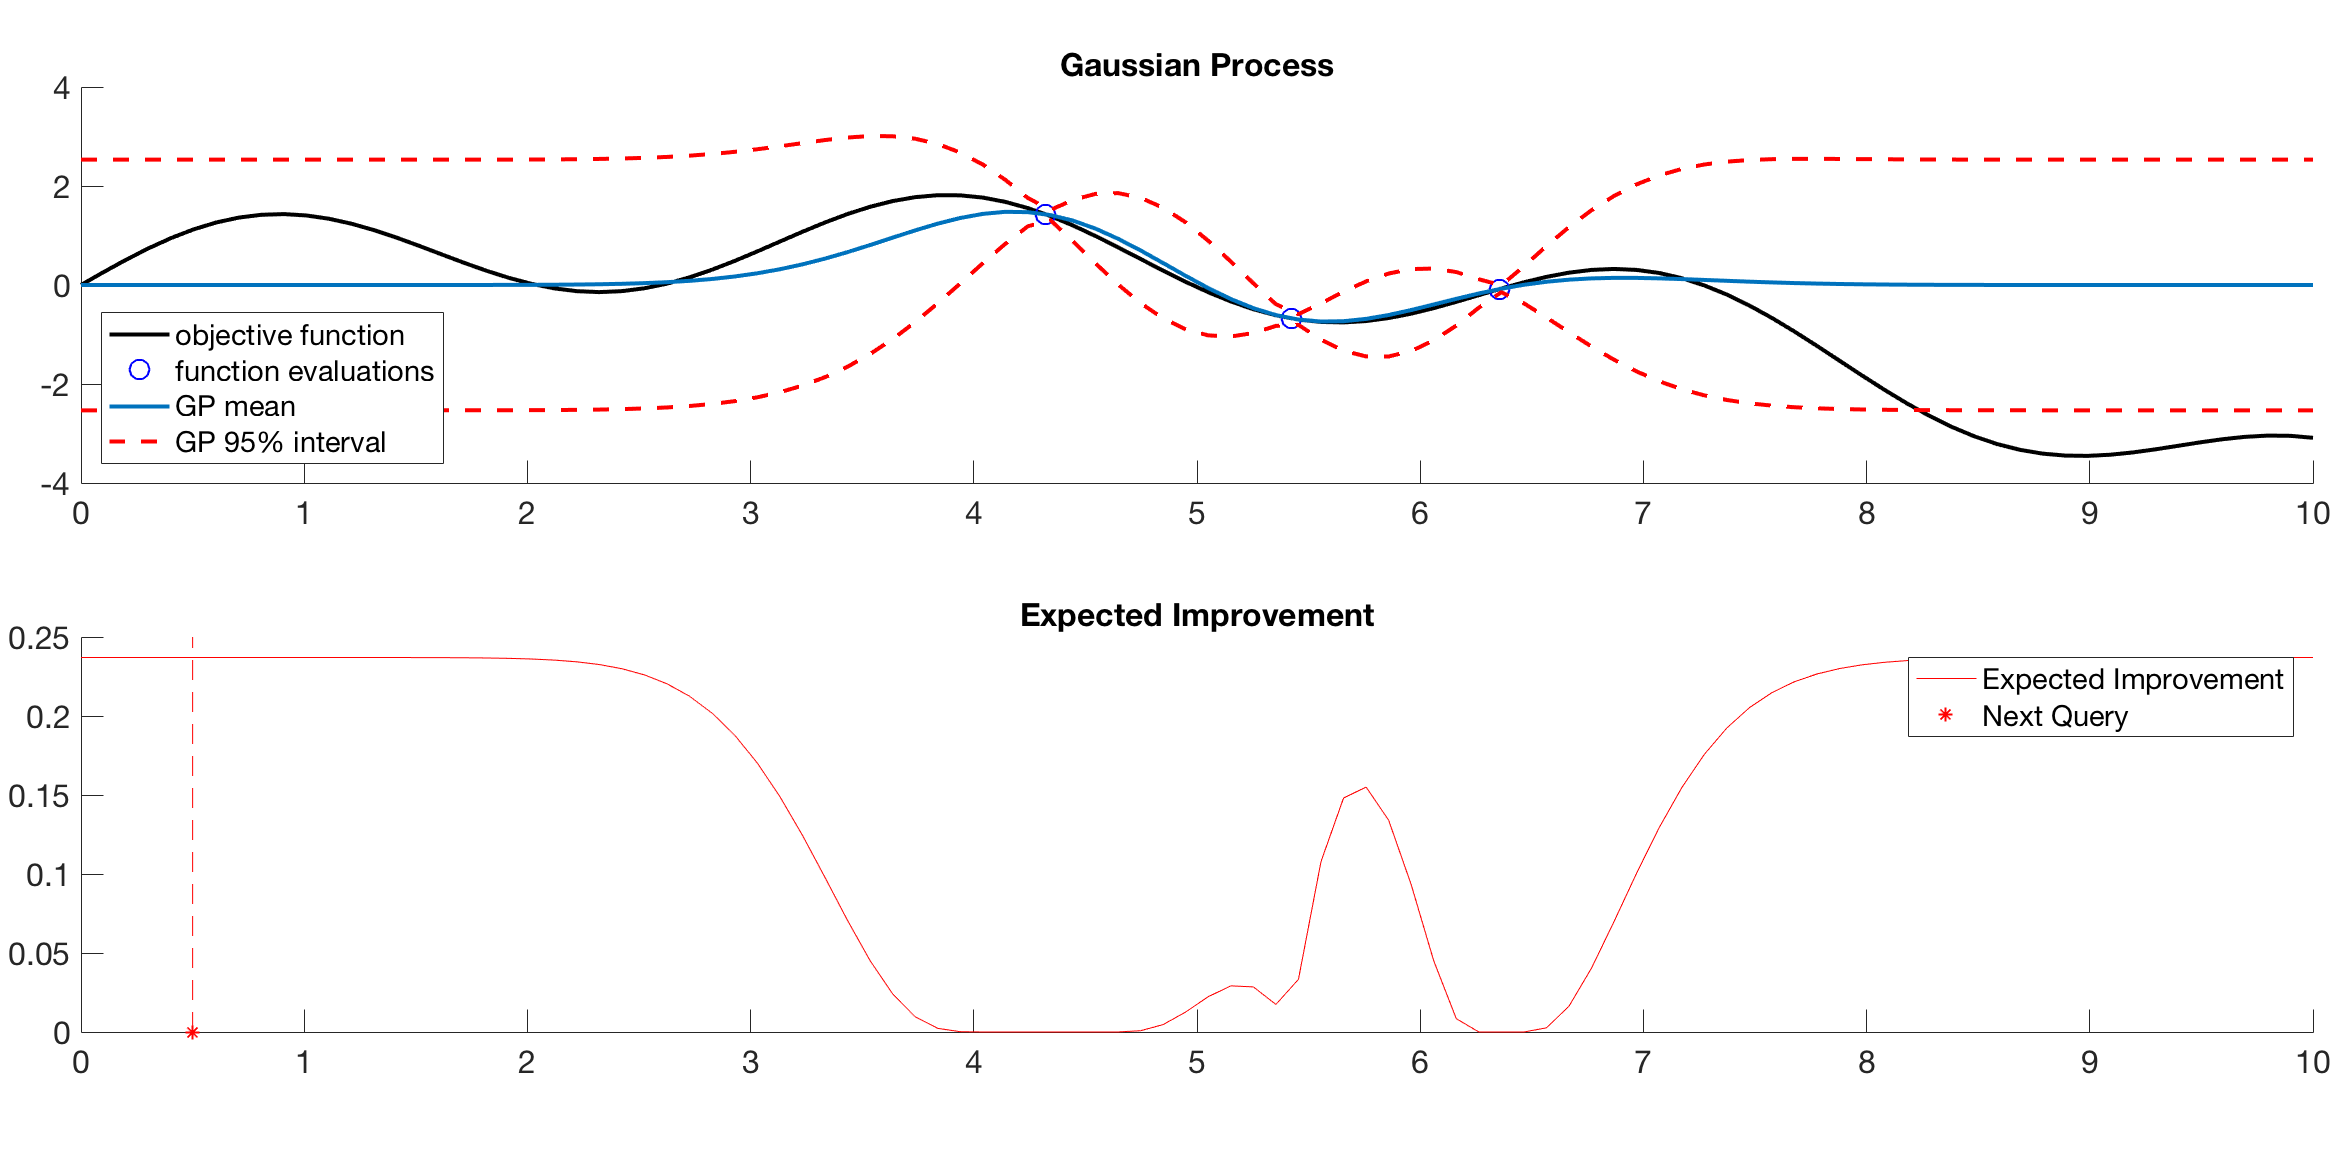
\includegraphics[width=.5\textwidth]{ei3.png}\hfill
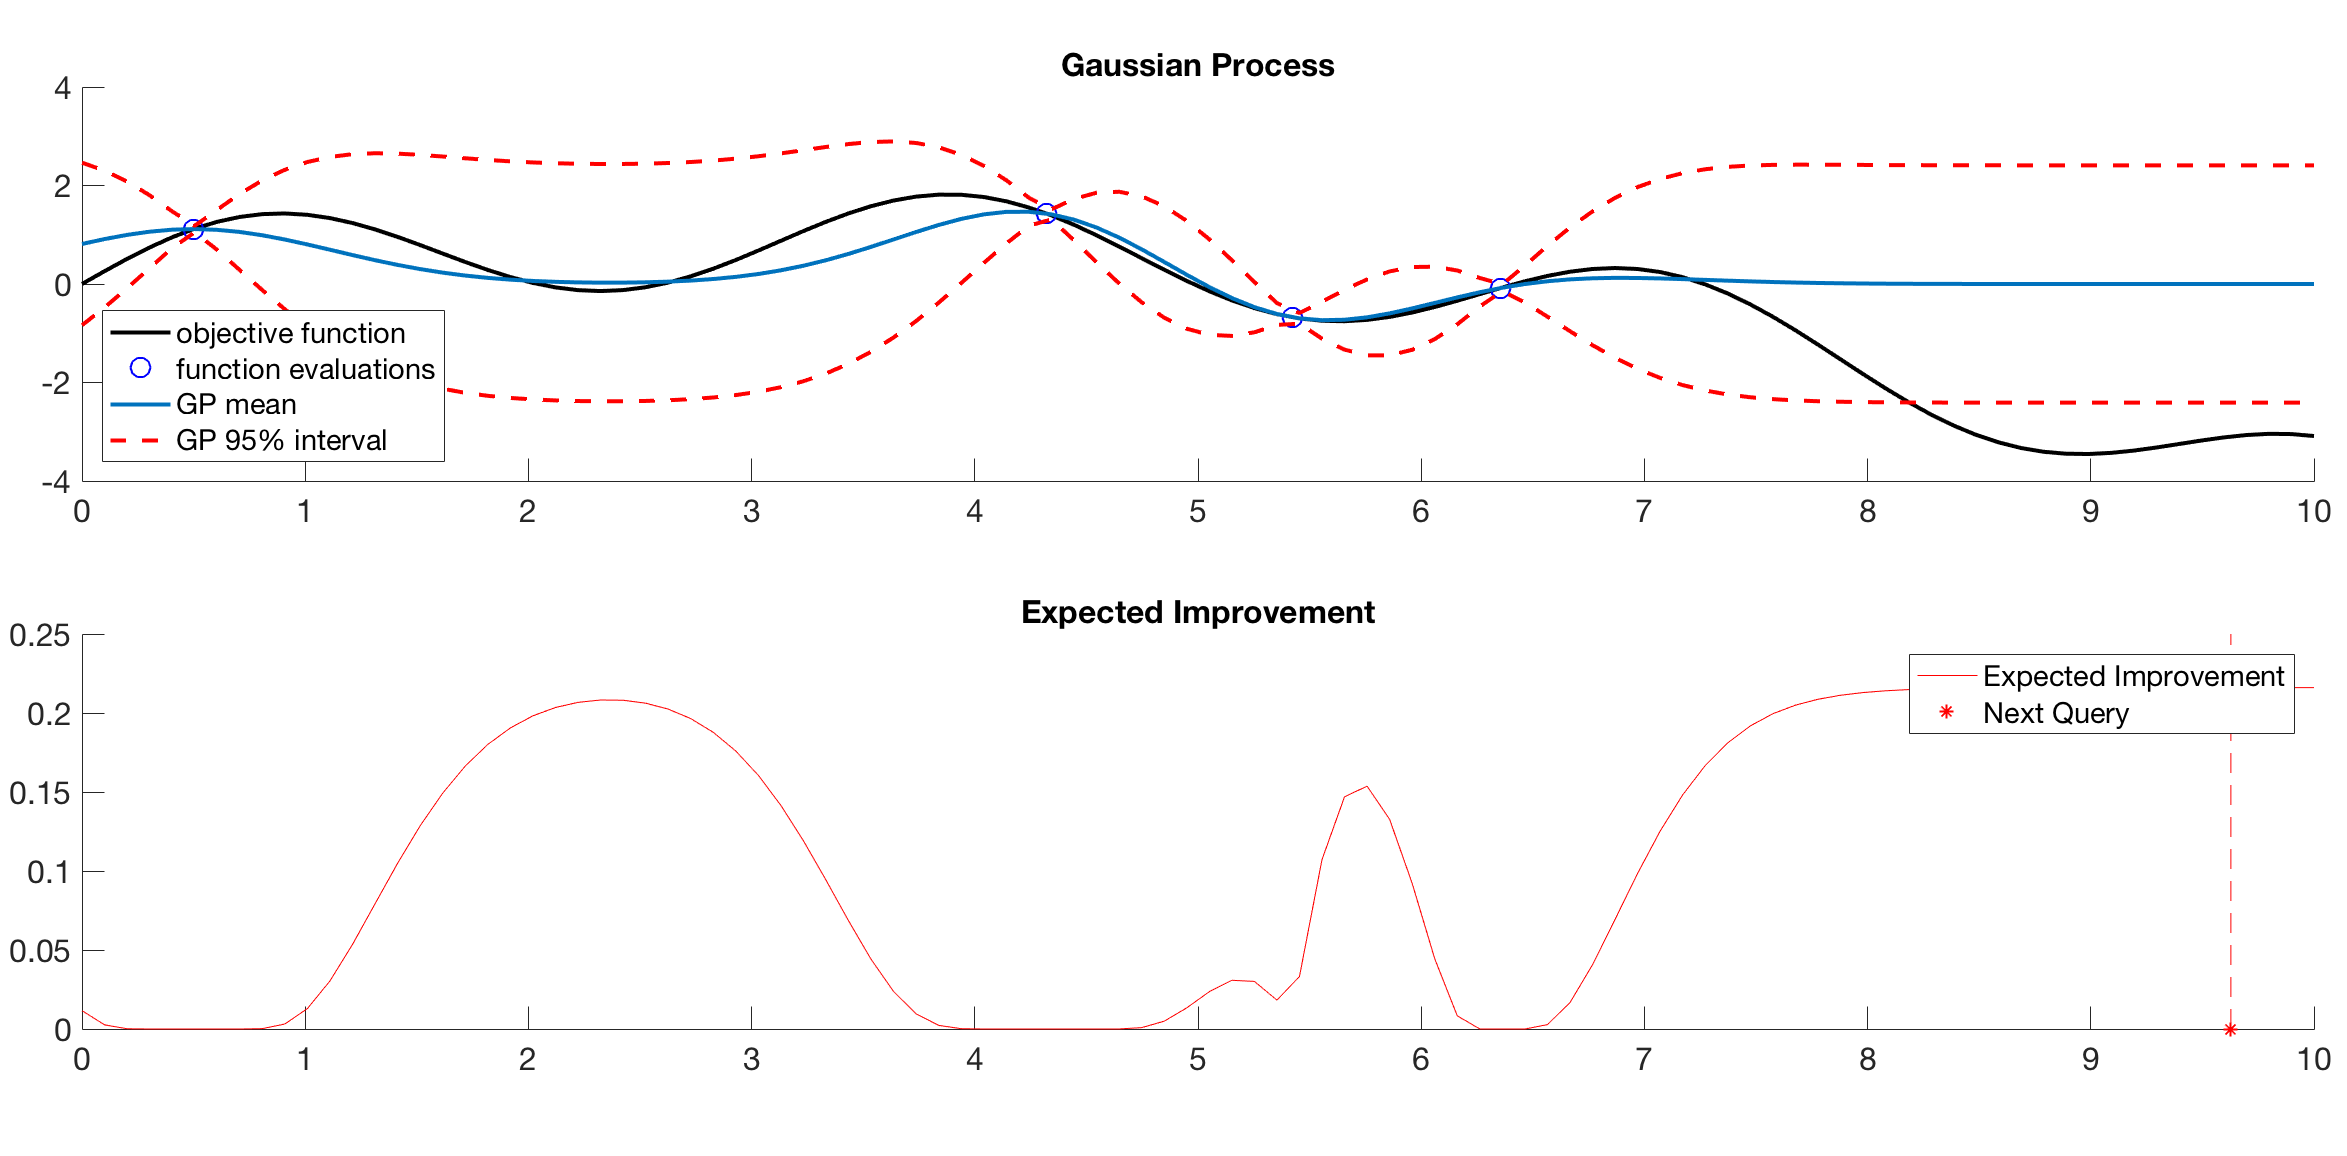
\includegraphics[width=.5\textwidth]{ei4.png}
\caption{Iterations 3 and 4}
\end{subfigure}
\caption{Four Iterations of Bayesian Optimization}
\label{fig:ei}
\end{sidewaysfigure}

%\chapter{Appendix to Chapter \ref{ch:2}}\label{cha:append-chapt-refch:2}
\chapter{Unscented Kalman Filter\footnote{\citet{Wan00theunscented}}}\label{ch:append-ukf}
The unscented transformation selects a representative set of points (sigma points) with associated weights to propagate through a nonlinear function. More formally, given an $N$-dimensional random variable $x$ with mean $\bar{x}$ and covariance $P_x$ we calculate the following sigma vectors 
\begin{equation}\label{eq:unscentedtransform}
\begin{aligned}
  \chi_0 &= \bar{x}\\
  \chi_i &= \bar{x} + (\sqrt{(N + \lambda)P_x})_i & i = 1, ..., N \\
  \chi_i &= \bar{x} - (\sqrt{(N + \lambda)P_x})_{i-N} & i = N + 1, ..., 2N\\
  W_0^{(m)} &= \lambda /(N + \lambda) \\
  W_0^{(c)} &= \lambda /(N + \lambda) + (1- \alpha^2 + \beta)\\
  W_i^m &= W_i^c = 1/\{(2(N + \lambda))\} & i = 1, ..., 2N,
\end{aligned}
\end{equation}
where $(\sqrt{(N + \lambda)P_x})_i$ represents the $i$th row of the matrix square root, $\lambda = \alpha^2(N + \kappa) - N$, and $\alpha$, $\kappa$, and $\beta$ are scaling parameters. For a given nonlinear function $y=g(x)$, an estimate for the mean and covariance are then
\begin{align}
\begin{split}
  \bar{y} &\approx \sum_{i=0}^{2N} W_i^{(m)}g(\chi_i)\\
  P_y &\approx \sum_{i=0}^{2N} W_i^{(c)}(g(\chi_i) - \bar{y})(g(\chi_i) - \bar{y})^T
\end{split}
\end{align}

Accurate to the second order, the Unscented Kalman Filter incorporates this transformation in it's $F$ and $H$ functions as follows:

\begin{algorithmic}
\State \textkeyword{Initial State Estimate and Covariance} $\hat{x}(0), P_{x}(0)$
\State \textkeyword{Define Augmented State } $x^a = [x^T \tab v^T \tab w^T]^T$
\State \textkeyword{Define Augmented Sigma Points } $\chi^a = [(\chi^x)^T  \tab (\chi^v)^T  \tab (\chi^w)^T]^T$
\State \textkeyword{Initial Augmented State Estimate } $\hat{x}^a(0) = [\hat{x}(0)^T  \tab 0  \tab 0]^T$
\State \textkeyword{Initial Augmented Covariance } $P^a(0) =
\begin{bmatrix}
	P_{x}(0) & 0 & 0\\
	0 & P_v & 0\\
	0 & 0 & P_w
\end{bmatrix}$ 
\For{t=1}{T}
  \State Using \ref{eq:unscentedtransform} Calculate Sigma Points $\chi^a(t)$ And Weights $W^{(m)}, W^{(c)}$
  \State Time Update:
  \begin{align*}
  	\chi_i^x(t\vert t-1) &= F(\chi_i^x(t-1), \chi_i^v(t-1), t-1)\\
  	\hat{x}(t\vert t-1) &= \sum_{i=0}^{2N} W_i^{(m)}\chi_i^x(t\vert t-1)\\
  	P_{x}(t\vert t-1) &= \sum_{i=1}^{2N} W_i^{(c)} \{\chi_i^x(t\vert t-1) - \hat{x}(t\vert t-1)\}\{\chi_i^x(t\vert t-1) - \hat{x}(t\vert t-1)\}^T\\
  	\mathbb{Z}_i(t\vert t-1) &= H(\chi_i^x(t\vert t-1), \chi_i^w(t-1), t-1)\\
  	\hat{z}(t\vert t-1) &= \sum_{i=1}^{2N} W_i^{(m)}\mathbb{Z}_i(t\vert t-1)
  \end{align*}
  \State Measurement Update:
  \begin{align*}
  	P_{y}(t\vert t-1) &= \sum_{i=1}^{2N}W_i^{(c)}\{\mathbb{Z}_i(t\vert t-1) - \hat{z}(t\vert t-1)\}\{\mathbb{Z}_i(t\vert t-1) - \hat{z}(t\vert t-1)\}^T\\
  	P_{xy}(t\vert t-1) &= \sum_{i=1}^{2N}W_i^{(c)}\{\chi_i^x(t\vert t-1) - \hat{x}(t\vert t-1)\}\{\chi_i^x(t\vert t-1) - \hat{x}(t\vert t-1)\}^T\\
  	K &= P_{xy}(t\vert t-1)P^{-1}_{y}(t\vert t-1)\\
  	\hat{x}(t) &= \hat{x}(t\vert t-1) + K(z(t) - \hat{z}(t\vert t-1))\\
  	P_{x}(t) &= P_{x}(t\vert t-1) - KP_{y}(t\vert t-1)K^T
  \end{align*}
\End
\end{algorithmic}

\chapter{Optimal Stopping Time Derivation}\label{thm:ost}
Define the process
\begin{align*}
	Z_n = \sum_{i=0}^{n-1} \lambda^ir(X_i) + \lambda^nJ_n(X_n)
\end{align*}
Then, we have
\begin{align*}
	\mathbb{E}[Z_{n+1} \vert X_n, X_{n-1}, ..., X_0] &= \sum_{i=0}^n \lambda^ir(X_i) + \lambda^{n+1}\mathbb{E}[J_{n+1}(X_{n+1})\vert X_n]\\
	&= \sum_{i=0}^{n-1} \lambda^ir(X_i) + \lambda^n(r(X_n) + \lambda\mathbb{E}[J_{n+1}(X_{n+1})\vert X_n])\\
	&\leq \sum_{i=0}^{n-1} \lambda^i r(X_i) + \lambda^nJ_n(X_n) = Z_n
\end{align*}
Since by definition $J_n(x) \geq g(x)$, we have
\begin{align*}
	\mathbb{E}[\sum_{i=0}^{\tau-1}\lambda^ir(X_i) + \lambda^{\tau}g(X_{\tau})] \leq \mathbb{E}[Z_{\tau}] \leq \mathbb{E}[Z_0] = J_0(X_0)
\end{align*}
for any stopping time $\tau \geq 0$. 

We now prove that $J_0(X_0)$ is exactly equal to $\mathbb{E}[Z_{\tau^*}]$ for optimal stopping time $\tau^*$. Consider the following for $0 \leq n < N$
\begin{align*}
	\mathbb{E}&[Z_{min(\tau^*, n+1)}\vert X_n, X_{n-1}, ..., X_0]\\
	&= 1_{\{\tau^* \leq n\}}Z_{\tau^*} + 1_{\{\tau^* > n\}}\mathbb{E}[Z_{n+1}\vert X_n, X_{n-1}, ..., X_0]\\
	&= 1_{\{\tau^* \leq n\}}Z_{\tau^*} + 1_{\{\tau^* > n\}}(\sum_{i=0}^n \lambda^ir(X_i) + \lambda^{n+1}\mathbb{E}[J_{n+1}(X_{n+1})\vert X_n])\\
	&= 1_{\{\tau^* \leq n\}}Z_{\tau^*} + 1_{\{\tau^* > n\}}(\sum_{i=0}^{n-1} \lambda^ir(X_i) + \lambda^nJ_n(X_n)) \tab (\tau^* > n\leftrightarrow J_n(X_n) = r(x) + \lambda\mathbb{E}[J_{n+1}(X_{n+1})])\\ 
	&= 1_{\{\tau^* \leq n\}}Z_{\tau^*} + 1_{\{\tau^* > n\}}Z_{n}\\
	&= Z_{min(\tau^*, n)}
\end{align*}
Then, it follows that
\begin{align*}
	J_0(X_0) &= \mathbb{E}[Z_0] = \mathbb{E}[Z_{min(\tau^*, 0)}] = ... = \mathbb{E}[Z_{min(\tau^*, N)}] = \mathbb{E}[Z_{\tau^*}]\\
			 &= \mathbb{E}[\sum_{i=0}^{\tau^* -1}\lambda^ir(X_i) + \lambda^{\tau^*}J_{\tau^*}(X_{\tau^*})] = \mathbb{E}[\sum_{i=0}^{\tau^* -1}\lambda^ir(X_i) + \lambda^{\tau^*}g(X_{\tau^*})]
\end{align*}
and $J_{\tau^*}(X_{\tau^*}) = g(X_{\tau^*})$ at $\tau^*$.

\chapter{Simulation Results}\label{ch:append-sims}
\end{appendices}


\end{document}
